%% Преамбула TeX-файла

% 1. Стиль и язык
\documentclass[utf8x, 12pt]{G7-32} % Стиль (по умолчанию будет 14pt)

% Остальные стандартные настройки убраны в preamble-std.tex
\sloppy

% 1. Настройки стиля ГОСТ 7-32
% Для начала определяем, хотим мы или нет, чтобы рисунки и таблицы нумеровались в пределах раздела, или нам нужна сквозная нумерация.
% А не забыл ли автор букву 't' ?
\EqInChapter % формулы будут нумероваться в пределах раздела
\TableInChapter % таблицы будут нумероваться в пределах раздела
\PicInChapter % рисунки будут нумероваться в пределах раздела

% 2. Добавляем гипертекстовое оглавление в PDF
\usepackage[
bookmarks=true, colorlinks=true, unicode=true,
urlcolor=black,linkcolor=black, anchorcolor=black,
citecolor=black, menucolor=black, filecolor=black,
]{hyperref}

% 3. Изменение начертания шрифта --- после чего выглядит таймсоподобно.
% apt-get install scalable-cyrfonts-tex

\IfFileExists{cyrtimes.sty}
    {
        \usepackage{cyrtimespatched}
    }
    {
        % А если Times нету, то будет CM...
    }


% 4. Прочие полезные пакеты.
\usepackage{underscore} % Ура! Теперь можно писать подчёркивание.
                        % И нельзя использовать подчёркивание в файлах.
                        % Выбирай, но осторожно.

\usepackage{graphicx}   % Пакет для включения рисунков

 % 5. Любимые команды
\newcommand{\Code}[1]{\textbf{#1}}

% 6. Поля
% С такими оно полями оно работает по-умолчанию:
% \RequirePackage[left=20mm,right=10mm,top=20mm,bottom=20mm,headsep=0pt]{geometry}
% Если вас тошнит от поля в 10мм --- увеличивайте до 20-ти, ну и про переплёт не забывайте:
\geometry{right=20mm}
\geometry{left=30mm}


% 7. Tikz
\usepackage{tikz}
\usetikzlibrary{arrows,positioning,shadows}

% 8 Листинги

\usepackage{listings}

% Значения по умолчанию
\lstset{
  basicstyle= \footnotesize,
  breakatwhitespace=true,% разрыв строк только на whitespacce
  breaklines=true,       % переносить длинные строки
%   captionpos=b,          % подписи снизу -- вроде не надо
  inputencoding=koi8-r,
  numbers=left,          % нумерация слева
  numberstyle=\footnotesize,
  showspaces=false,      % показывать пробелы подчеркиваниями -- идиотизм 70-х годов
  showstringspaces=false,
  showtabs=false,        % и табы тоже
  stepnumber=1,
  tabsize=4,              % кому нужны табы по 8 символов?
  frame=single
}

% Стиль для псевдокода: строчки обычно короткие, поэтому размер шрифта побольше
\lstdefinestyle{pseudocode}{
  basicstyle=\small,
  keywordstyle=\color{black}\bfseries\underbar,
  language=Pseudocode,
  numberstyle=\footnotesize,
  commentstyle=\footnotesize\it
}

% Стиль для обычного кода: маленький шрифт
\lstdefinestyle{realcode}{
  basicstyle=\scriptsize,
  numberstyle=\footnotesize
}

% Стиль для коротких кусков обычного кода: средний шрифт
\lstdefinestyle{simplecode}{
  basicstyle=\footnotesize,
  numberstyle=\footnotesize
}

% Стиль для BNF
\lstdefinestyle{grammar}{
  basicstyle=\footnotesize,
  numberstyle=\footnotesize,
  stringstyle=\bfseries\ttfamily,
  language=BNF
}

% Определим свой язык для написания псевдокодов на основе Python
\lstdefinelanguage[]{Pseudocode}[]{Python}{
  morekeywords={each,empty,wait,do},% ключевые слова добавлять сюда
  morecomment=[s]{\{}{\}},% комменты {а-ля Pascal} смотрятся нагляднее
  literate=% а сюда добавлять операторы, которые хотите отображать как мат. символы
    {->}{\ensuremath{$\rightarrow$}~}2%
    {<-}{\ensuremath{$\leftarrow$}~}2%
    {:=}{\ensuremath{$\leftarrow$}~}2%
    {<--}{\ensuremath{$\Longleftarrow$}~}2%
}[keywords,comments]

% Свой язык для задания грамматик в BNF
\lstdefinelanguage[]{BNF}[]{}{
  morekeywords={},
  morecomment=[s]{@}{@},
  morestring=[b]",%
  literate=%
    {->}{\ensuremath{$\rightarrow$}~}2%
    {*}{\ensuremath{$^*$}~}2%
    {+}{\ensuremath{$^+$}~}2%
    {|}{\ensuremath{$|$}~}2%
}[keywords,comments,strings]

% Подписи к листингам на русском языке.
\renewcommand*\thelstnumber{\oldstylenums{\the\value{lstnumber}}}
\renewcommand\lstlistingname{\cyr\CYRL\cyri\cyrs\cyrt\cyri\cyrn\cyrg}
\renewcommand\lstlistlistingname{\cyr\CYRL\cyri\cyrs\cyrt\cyri\cyrn\cyrg\cyri}

% Произвольная нумерация списков.
\usepackage{enumerate}


\begin{document}

\frontmatter % выключает нумерацию ВСЕГО; здесь начинаются ненумерованные главы: реферат, введение, глоссарий, сокращения и прочее

% Команды \breakingbeforechapters и \nonbreakingbeforechapters
% управляют разрывом страницы перед главами.
% По-умолчанию страница разрывается.

% \nobreakingbeforechapters
% \breakingbeforechapters

% % Также можно использовать \Referat, как в оригинале
\begin{abstract}
Это пример каркаса расчётно-пояснительной записки, желательный к использованию в РПЗ проекта по курсу РСОИ.

Дополняет краткое пособие по графике в Latex.  Данный опус, как и более новые версии этого документа, можно взять по адресу (\url{http://sevik.ru/latex}). Минимально необходимые пакеты Latex, которые должны стоять: mathtext, amssymb, amsmath, icomma, longtable, graphicx, underscore, cmap, hyperref.

Текст в документе носит совершенно абстрактный характер.
\end{abstract}

%%% Local Variables: 
%%% mode: latex
%%% TeX-master: "rpz"
%%% End: 


\tableofcontents

\Defines % Необходимые определения. Вряд ли понадобться
\begin{description}
\item[Распределённый] Слово, которое нельзя употреблять. Но надо протестировать длинные строки в глоссарии.
\end{description}

%%% Local Variables:
%%% mode: latex
%%% TeX-master: "rpz"
%%% End:

\Abbreviations %% Список обозначений и сокращений в тексте
\begin{description}
\item[АИС] Автоматизированная информационная система. Но надо протестировать длинные строки в определениях.
\end{description}

%%% Local Variables:
%%% mode: latex
%%% TeX-master: "rpz"
%%% End:


\Introduction

В настоящее время роботы вошли в жизнь человека в разных областях, но до сих пор нет четкого разделения среди робототехнических устройств, а также единой программной платформы. Разные производители делают разные и абсолютно несовместимые аппаратные средства. Технологии и инструменты затачиваются каждый раз под конкретные проблемы, их практически невозможно повторно использовать. Основной камень преткновения при создании роботов — искусственный интеллект. 

Какие проблемы стоят перед современной робототехникой?

\begin{itemize}
\item надёжная и доступная механика;
\item емкие и компактные элементы питания;
\item мощная и малопотребляющая вычислительная система;
\item точные и доступные датчики;
\item интеллектуальная система управления.
\end{itemize}

В рамках данной дипломной работы мы попытаемся решить задачу, которая лежит на стыке 3ех проблем: механики, вычислительной системы и системы управления.
Мы сформируем у робота мелкую моторику, которая будет заключаться в том, что мы научим робота писать простые символы. Другими словами, сформируем основы графомоторных навыков у робота на примере решения игры в Судоку.

Мы будем использовать робота LEGO MINDSTORMS [NXT] 2, который достаточно распространен у любителей робототехники.

Проблемы, которые придется нам решить в ходе данной дипломной работы это малое количество flash-памяти на роботе (256Кб) и недостаточная разрешающая способность блока с камерой (CAM-NXT).

Последовательность действий для  получения решения:
\begin{enumerate}
\item сфотографировать изображение;
\item распознать изображение;
\item сформировать решение.
\end{enumerate}
Для выполнения шага 1 и 2 нам не хватит встроенной памяти робота, так он не в состоянии даже сохранить фотографию в нужном нам качестве, поэтому решение данной задачи мы перенесем на внешнее мобильное устройство под управлением операционной системы Android. На телефоне мы распознаем изображение и отправим роботу посредством канала Bluetooth.

На выходе мы получаем:
\begin{enumerate}
\item простейшую систему распознавания цифр на телефоне, под управлением ОС Android;
\item протокол обмена между роботом и мобильным устройством;
\item система решения Судоку на роботе;
\item система отрисовки на бумаге полученного решения.
\end{enumerate}

\mainmatter % это включает нумерацию глав и секций в документе ниже

\chapter{Аналитический раздел}
\label{cha:analysis}
%
% % В начале раздела  можно напомнить его цель
%
В данном разделе производится анализ процессов распознавания изображения, передачи распознанного изображения, приема изображения и  решения решение его на роботе.
Производится анализ подсистем, входящих в реализуемы программно-аппаратный комплекс, формируются требования к создаваемой системе, выделяются функции её подсистем и описывается взаимодействие между ними.

\section{Общее описание системы}
В рамках данной дипломной работы разрабатывается автономный программно-аппаратный комплекс предоставляющий полный цикл для передачи и распознавания информации, для функционирования которой необходимо спроектировать все подсистемы программного комплекса и способы их взаимодействия.

Для достижения поставленной цели необходимо спроектировать и разработать следующие компоненты системы:
\begin{enumerate}
\item разработать систему распознавания изображения;
\item разработать протокол обмена между роботом и мобильным устройством;
\item разработать систему решения Судоку;
\item разработать систему отрисовки на бумаге полученного решения.
\end{enumerate}

\begin{figure}
  \centering
  \includegraphics[width=\textwidth]{inc/dia/analysis1-1}
  \caption{Схема работы комплекса}
  \label{fig:fig01}
\end{figure}


Так же для удобства и простоты использования комплекса необходимо разработать мобильное приложение и протокол обмена между мобильным устройством и роботом, для того, чтобы стандартизировать сообщения и разрабатывать приложения для любых внешних платформ.

\begin{figure}
  \centering
  \includegraphics[width=\textwidth]{inc/dia/analysis1-2}
  \caption{Компоненты системы}
  \label{fig:fig02}
\end{figure}

\section{Цель и задачи}
Целью данной работы является решение головоломки Судоку роботом и вывод решения роботом на лист бумаги.


Входные данные.
\begin{itemize}
\item головоломка судоку на листе бумаги.
\end{itemize}

Выходные данные.
\begin{itemize}
\item решение головоломки на листе бумаги.
\end{itemize}

Последовательность действий для  получения решения:
\begin{enumerate}
\item сфотографировать изображение;
\item распознать изображение;
\item сформировать решение.
\end{enumerate}
Для выполнения шага 1 и 2 нам не хватит встроенной памяти робота, так он не в состоянии даже сохранить фотографию в нужном нам качестве, поэтому решение данной задачи мы перенесем на внешнее мобильное устройство под управлением операционной системы Android. На телефоне мы распознаем изображение и отправим роботу посредством канала Bluetooth.

На выходе мы получаем:
\begin{enumerate}
\item простейшую систему распознавания цифр на телефоне, под управлением ОС Android;
\item протокол обмена между роботом и мобильным устройством;
\item система решения Судоку на роботе;
\item система отрисовки на бумаге полученного решения.
\end{enumerate}

% Обратите внимание, что включается не ../dia/..., а inc/dia/...
% В Makefile есть соответствующее правило для inc/dia/*.pdf, которое
% берет исходные файлы из ../dia в этом случае.

\section{Подсистема предоставления доступа к данных}

\subsection{Общие представления о системе}

Главной задачей разрабатываемой системы является предоставление доступа сторонним приложениям доступ к массивам данных, хранящихся на серверах системы. Как известно, "чтобы купить что-нибудь ненужное, нужно сначала купить что-нибудь ненужное", и эту задачу призвана решить первая рассматриваемая подсистема - подсистема сбора данных. Второй важнейшей задачей является сохранение данных, а так же и непосредственная передача клиенту. Эту проблему призвано решить вторая рассматриваемая подсистема.

Очевидно, что в качестве сердца данной подсистемы выступает некоторая база данных, которую необходимо наполнить данными, а затем и предоставить доступ к этим данным. Для решения это задачи должно быть разработано приложения, предоставляющий некоторый интерфейс для доступа к базе данных, так как прямой доступ к базе крайне нежелателен, а в некоторых случаях даже опасен. Такой интерфейс и будет предоставлять второе приложение.

\begin{figure}[ht!]
 \centering 
 
\includegraphics[width=\textwidth]{inc/raster/sample.jpg} 
 \caption{A simple caption} 
 \label{overflow} 
\end{figure}



\section{Какой-то последний раздел}
Проблемы, которые придется нам решить в ходе данной дипломной работы это малое количество flash-памяти на роботе (256Кб) и недостаточная разрешающая способность блока с камерой (CAM-NXT).

%%% Local Variables:
%%% mode: latex
%%% TeX-master: "rpz"
%%% End:

\chapter{Конструкторский раздел}
\label{cha:design}

В данном разделе на основе проведенного анализа описывается взаимодействие между подсистемами, выделяются основные составляющие в каждой системе и проектируется их взаимодействие.

\section{Конструкция робота}


\section{Подсистема распознавания}
\subsection{Основные задачи}
В данной секции сформируем опишем уже формализованный список задач, которые нам необходимо будет произвести над картинкой.
Модно выделить основные моменты при данной системой:
\begin{enumerate}
  \item сфотографировать;
  \item перевести изображение в черно-белые цвета;
  \item определить угол наклона изображения;
  \item определить сетку;
  \item распознать и разместить цифры в сетке;
  \item скорректировать распознавание под правила Судоку.
\end{enumerate}

\subsection{Фотографирование}
Данный процесс делается стандартными средствами Android API. Необходимо лишь получить изображение из камеры или галереи, после чего передать изображение на обработку.

\subsection{Конвертация в монохромное изображение}
Каждое приложение с компьютерным зрением начинает с конвертации цветного (или чёрно-белого) изображения в монохромное. В будущем, возможно, будет какой-то алгоритм, который будет использовать цвета, но сегодня приложения компьютерного зрения работают с монохромными изображениями (они дальтоники).
Самый простой метод для конвертации изображения – это общий порог. Предположим, что у вас есть пиксель с цветом RGB (200, 200, 200). Так как интенсивность компонент изменяется от 0 до 255, то пиксель очень яркий. Выбрав порог, как половину интенсивности: 256/2=128, мы получим, что наш пиксель должен стать белым. Но общий порог редко используется в настоящих приложениях, так как он малополезен. Куда более полезен алгоритм локального порога.

На рис.~\ref{fig:fig21} показаны оригинальное фото (1), фото после обработки с общим порогом (2) и адаптивным порогом (3) .

\begin{figure}[ht!]
  \centering
  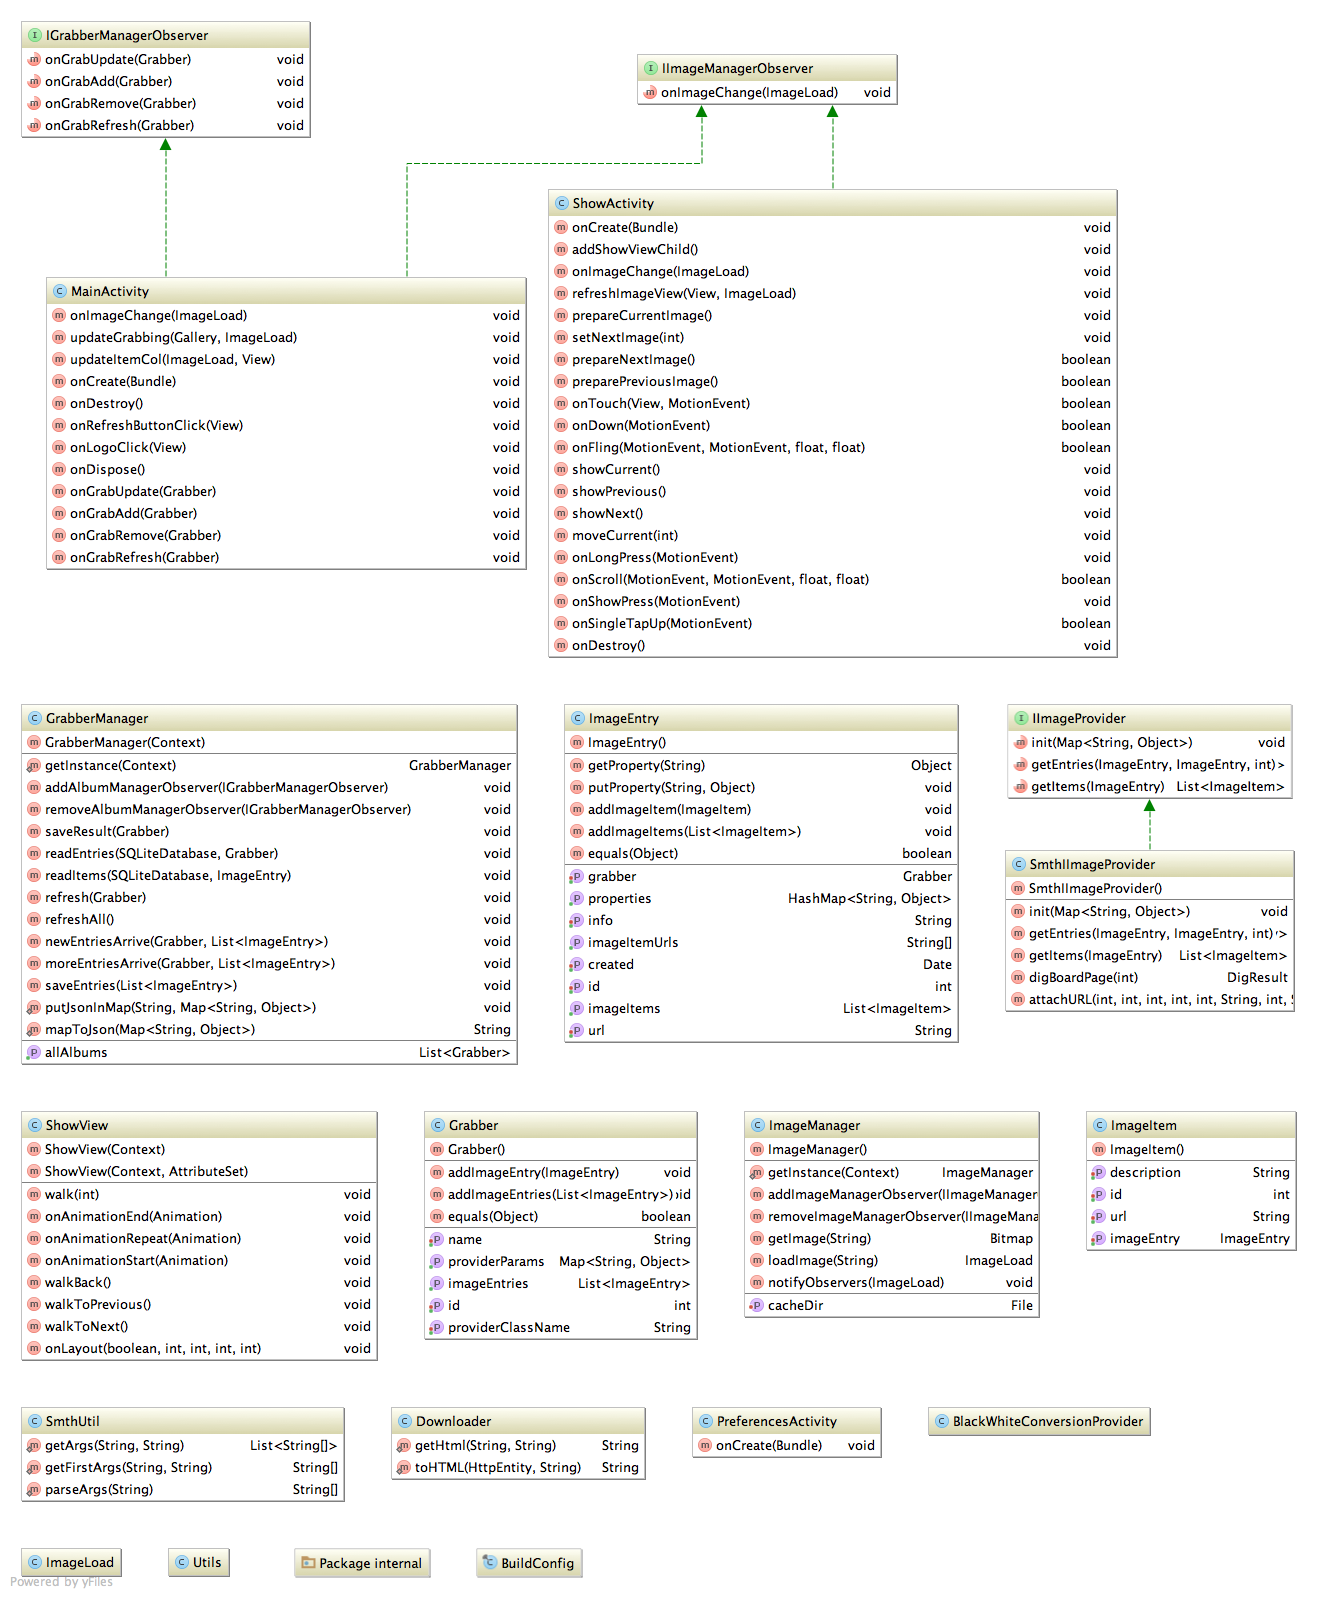
\includegraphics[width=\textwidth]{inc/raster/design2-1.png}
  \caption{Пороги при создании монохромного изображения}
  \label{fig:fig21}
\end{figure}

Для правильной конвертации изображения в монохромное, мы будем использовать адаптивный выбор порога. Он не использует фиксированное значение порога в 128. Вместо этого, он считает порог для каждого пикселя отдельно. Он берёт квадрат со стороной в ${l}$ пикселей и с центром в нашем пикселе и суммирует интенсивность всех точек. Среднее значение интенсивности и будет являться порогом для данного пикселя. Формула интенсивности для текущего пикселя: $\text{порог}=\frac{\text{сумма}}{l^2}$. Если интенсивность нашего пикселя выше порогового значения, то он конвертируется в белый, если же нет, то в чёрный. На изображении ниже пиксель, для которого определяется порог, отмечен красным. И эти подсчёты производятся для каждого пикселя. Поэтому данный шаг является таким медленным, ведь алгоритм требует $\text{ширина} * \text{порог} *{l^2}$ чтений пикселя изображения. Схема показана на рис.~\ref{fig:fig22}

\begin{figure}[ht!]
  \centering
  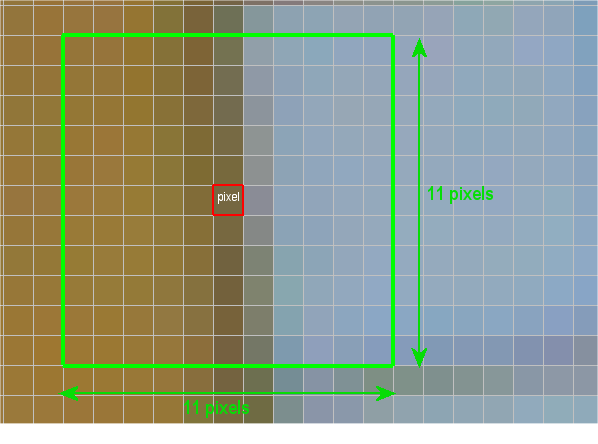
\includegraphics[width=0.7\textwidth]{inc/raster/design2-2.png}
  \caption{Адаптивный выбор порога при создании монохромного изображения}
  \label{fig:fig22}
\end{figure}

\subsubsection{Целочисленная форма}
\begin{figure}[ht!]
  \centering
  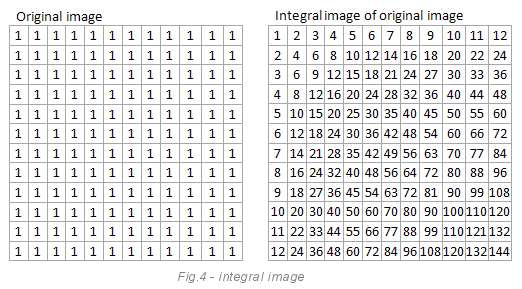
\includegraphics[width=\textwidth]{inc/raster/design2-3.png}
  \caption{Целочисленная форма}
  \label{fig:fig23}
\end{figure}

Этот шаг может быть оптимизирован с помощью использования «Целочисленной формы». Целочисленная форма – это массив целых чисел с размерами изображения. Допустим у нас есть область  на рис.~\ref{fig:fig23} $12{*}12$, где интенсивность пикселей равна $1$ (в реальном мире так не бывает), целочисленный образ – это сумма всех пикселей с левого верхнего до текущего (правого нижнего).

\begin{figure}[ht!]
  \centering
  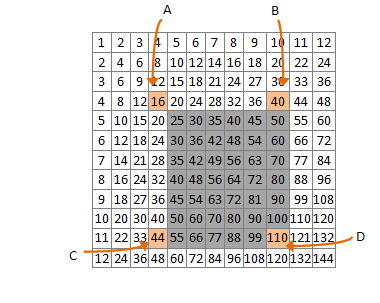
\includegraphics[width=0.6\textwidth]{inc/raster/design2-4.png}
  \caption{Целочисленная форма в области}
  \label{fig:fig24}
\end{figure}
Следующий рис.~\ref{fig:fig24} демонстрирует, чем может быть полезен целочисленный образ. Целью является посчитать сумму пикселей в сером прямоугольнике. 
Формула: $\text{сумма}=D{-}C{-}B{+}A$ . В нашем случае: $110-44-40+16=42$.

Вместо чтения всех пикселей из серого прямоугольника (который может быть намного больше, чем в примере), нам необходимо всего лишь одно чтение памяти. Это значительная оптимизация алгоритма. Но даже с ней, конвертация изображения в монохромное является очень тяжёлой. 


\subsubsection{Определение угла поворота}
Камера не сканер. И картинка никогда не будет идеально ровно, а значит в порядке вещей немного скошенное и повёрнутое изображение. Чтобы определить угол поворота, мы будем пользоваться фактом, что изображение с судоку всегда имеет горизонтальные и вертикальные линии. Мы будем определять самые выразительные и жирные линии рядом с центром изображения. Самые выразительные линии не подвержены зашумлению.

Алгоритм нахождения монохромных линий на изображении называется преобразованием Хафа. 

\begin{equation}
\label{f:angleOfRotation}
y = \frac{x * \cos \theta + rho}{\sin \theta}
\end{equation}
где $\theta$~--- угол линии; $rho$~--- является расстоянием от линии до центра координат (0, 0). На риc.~\ref{fig:fig25}

\begin{figure}[ht!]
  \centering
  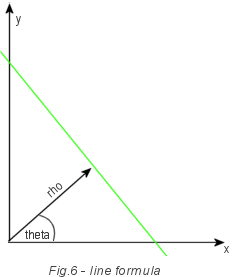
\includegraphics[width=0.5\textwidth]{inc/raster/design2-5.png}
  \caption{Угол поворота}
  \label{fig:fig25}
\end{figure}

Важным является то, что линия может быть описана всего двумя переменными: углом наклона и расстоянием до центра координат. 

Алгоритм проходит по всем пикселям в монохромном изображении, пропуская белые пиксели. Когда он попал на чёрный пиксель, то пытается «нарисовать» всевозможные линии, проходящие через этот пиксель с шагом в 1 градус. Это означает, что каждый пиксель имеет 180 воображаемых линий, проходящих через него, потому что углы 180-360 являются копиями линий с углами 0-180 градусов. 

Это множество воображаемых линий называется накопителем, двумерным массивом с размерностями $\theta$ и $rho$, которые были в формуле выше. Каждая воображаемая линия представлена одним значением в накопителе. Кстати, метод называется преобразованием, потому что он преобразовывает линии из $(x, y)$ в массив $(\theta, rho)$. Каждая воображаемая линия добавляет значение в накопитель, повышая вероятность того, что воображаемая линия совпадает с реальной. По аналогии с голосованием. Настоящие линии имеют больше всего «голосов». 

После того, как все пиксели и их 180 воображаемых линий «проголосовали», мы должны найти максимальное значение в накопителе. (Накопителем он называется потому что накапливает голоса) Победителем голосования является самая выразительная линия. Её параметра $\theta$ и $rho$ могут использоваться с помощью формулы выше чтобы нарисовать её. 

На следующем риc.~\ref{fig:fig26} приведён небольшой пример. Слева мы имеем линию, состоящую из трёх пикселей. Вы точно знаете, что это диагональная линия слева направо, но для компьютера это не так очевидно. 
\begin{figure}[ht!]
  \centering
  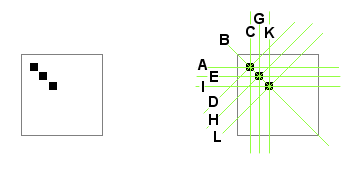
\includegraphics[width=0.6\textwidth]{inc/raster/design2-6.png}
  \caption{Определение нужной линии}
  \label{fig:fig26}
\end{figure}

Посмотрев на это изображение, можно понять, как же работает обнаружение линий. Алгоритм преобразования Хафа пропускает белые пиксели. На каждом чёрном пикселе он рисует четыре воображаемых зелёных линии (на самом деле их 180, но для простоты мы возьмём четыре), проходящие через текущий пиксель. Первый пиксель голосует за линии $A$, $B$, $C$ и $D$. Второй пиксель голосует за линии $E$, $B$, $G$, $H$. Третий за $I$, $B$, $K$, $L$. За линию $B$ проголосовали все три пикселя, а остальные линии получили всего по одному голосу. Таким образом, линия $B$ победила в голосовании.

\begin{figure}[ht!]
  \centering
  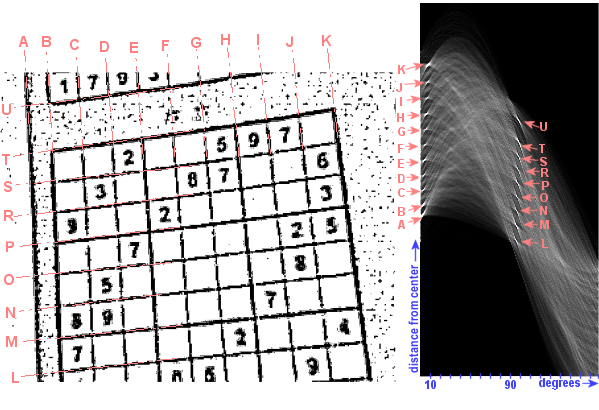
\includegraphics[width=0.8\textwidth]{inc/raster/design2-7.png}
  \caption{"Голосование" за линию}
  \label{fig:fig27}
\end{figure}
Следующий риc.~\ref{fig:fig27} является более сложным примером. Слева мы видим сетку судоку, а справа массив накопителя после прохождения по изображению алгоритма преобразования Хафа. Яркие светлые области являются линиями, которые получили много голосов. Темнота означает, что у нас нет шанса найти линию с такими параметрами на изображении. Сконцентрируемся только на ярких точках. Каждая линия $A-U$ имеет яркую точку в накопителе. Вы можете видеть, что все линии слегка повёрнуты (примерно на 6 градусов). Линия $A$ меньше повёрнута, чем линия $К$. Потому что изображение не только повёрнуто, но и скошено. Также, если вы посмотрите внимательнее, то увидите, что линии $А$ и $В$ ближе друг к другу, чем $В$ и $С$. Это можно заметить на обоих изображениях.

Преобразование Хафа важно понять, если вы хотите заниматься распознаванием образов. Концепция виртуальных линий, которые могут быть реальными с помощью голосования, может быть распространена на любую геометрическую фигуру. Линия – простейшая из них, поэтому является самой простой для понимания. 

Если вам надо найти окружность, то понадобится накопитель с тремя размерностями: $x$, $y$ и $r$. Где $x$ и $y$ являются координатами центра нашей окружности, а $r$ радиусом.

Преобразование Хафа может быть оптимизировано ограничением области и возможных углов исходного изображения. Нам не надо анализировать все линии, только те, что близки к центру. В нашем случае, именно от них мы и можем отталкиваться.

\subsubsection{Определение сетки}

Для получения чисел из сетки судоку, нам надо определить, а где же наша сетка начинается и кончается. Эта часть является простейшей частью для человеческого мозга, но самой сложной для автоматического распознавания. Почему? Почему бы не использовать линии, найденные с помощью преобразования Хафа в предыдущем шаге? В них слишком много лишних данных. На изображении будет слишком много лишних линий. 

Пример можно увидеть, посмотрев на риc.~\ref{fig:fig28}.
\begin{figure}[ht!]
  \centering
  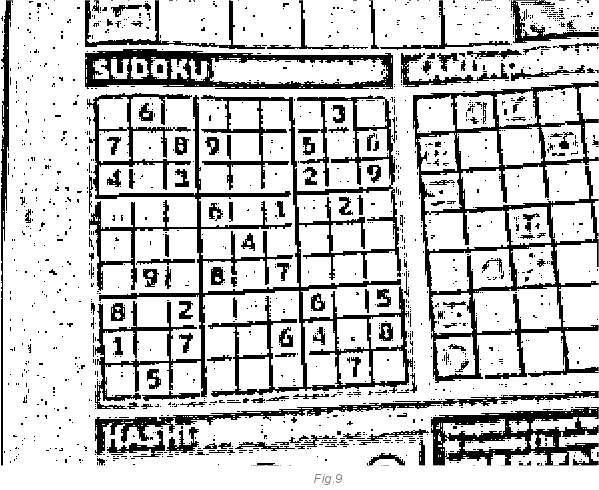
\includegraphics[width=0.8\textwidth]{inc/raster/design2-8.png}
  \caption{Зашумленное изображение}
  \label{fig:fig28}
\end{figure}

При автоматическом распознавании очень сложно определить, какие линии относятся к необходимым нам, а какие являются всего лишь информационным шумом. Где конец нашей сетки и начало следующей.

\begin{figure}[ht!]
  \centering
  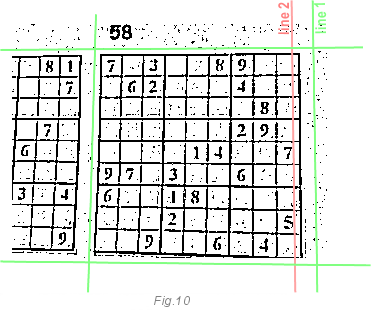
\includegraphics[width=0.8\textwidth]{inc/raster/design2-9.png}
  \caption{Отбрасывание информационного шума}
  \label{fig:fig29}
\end{figure}

Чтобы решить эту проблему, мы не будем определять чёрные линии. Вместо этого, мы будем определять белые области вокруг сетки. На  риc.~\ref{fig:fig29}, вы можете увидеть это. Зелёная линия 1 никогда не пересекается с чёрными пикселями в то время, как линия 2 делает это 10 раз. Это означает, что за сеткой скорее находится линия 1, нежели линия 2. Просто подсчитав, сколько раз зелёная линия пересекает чёрные пиксели, мы можем сделать вывод, что она находится за границей сетки. Достаточно просто подсчитать как много переходов с белого на чёрный пиксель под линией. Кстати, вам не надо пробегаться по каждой линии, достаточно выполнять эти действия каждую третью линию для увеличения скорости выполнения.


После того, как мы определили границы, запустим алгоритм преобразования Хафа чтобы точно определить линии сетки. До сих пор мы не заботились о перекосах и других дефектах изображения. Только об угле поворота. Этот шаг исправит это. Путём запуска преобразования Хафа, мы получим точные положения линий сетки. Это поможет определить числа в сетке.

Этот шаг может быть более устойчивым к шуму.

\subsection{Модуль OCR}
После того, как мы определили, где должны находиться числа, нам необходимо распознать их. Это относительно легко. В алфавите только цифры от 1 до 9.

Теория. Каждый алгоритм распознавания имеет три шага:
\begin{enumerate}
  \item определение необходимых признаков;
  \item тренировка;
  \item классификация (распознавание в реальности).
\end{enumerate}

Определение необходимых признаков является частью разработки приложения. Например, цифра один тонкая и высокая. Именно это и отличает её от остальных. Цифра 8 имеет две окружности, в верхней половине и в нижней, и т. д. 

Определение необходимых признаков может быть трудной и не интуитивной работой, в зависимости от того, что надо распознать. Например, что необходимо для распознавания чьего-то лица? Не любого, а какого-то конкретного.

\subsubsection{Зоны}
В нашем приложении был использован способ плотности зон. Следующим шагом (Это должно быть сделано заранее) является тренировка приложения на цифры от 1 до 9. Образцы эти изображения в каталоге хранятся в системе. Они уменьшены до размера 5х5, нормализованы и хранятся в статическом массиве \Code{OCRDigit::m_zon[10][5][5]}, который выглядит примерно так как на рис.~\ref{fig:fig210}:

\begin{figure}[ht!]
  \centering
  
\includegraphics[width=\textwidth]{inc/raster/design2-10.png}
  \caption{Нормализованные и уменьшенные образцы изображений}
  \label{fig:fig210}
\end{figure}

Уменьшение до размеров 5х5 называется зоннированием или разбивкой на зоны. Массив выше называется плотностью функции.
Нормализация значит, что плотность варьируется от 0 до 1024. Без нормализации зоны нельзя сравнивать корректно.

Что происходит во время выполнения программы: когда цифра получена из исходного изображения, она уменьшается до размера 5х5. После этого каждый её пиксель сравнивается с каждым пикселем из девяти цифр из тренированного массива. Целью является найти цифру с минимальным различием. 

\begin{figure}[ht!]
  \centering
  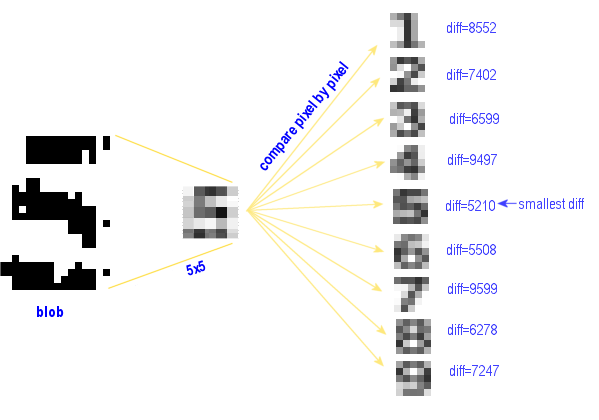
\includegraphics[width=\textwidth]{inc/raster/design2-11.png}
  \caption{Процесс уменьшения и сравнения с образцом}
  \label{fig:fig211}
\end{figure}
Этот метод инвариантен к размеру изображения, так как в любом случае мы используем зоны 5х5. Он чувствителен к поворотам, но мы уже позаботились об этом раньше. Проблема в том, что он чувствителен к позиции и смещению, а также не работает с негативами (белым по чёрному) и перевёрнутыми вверх тормашками цифрами. Изображен на на рис.~\ref{fig:fig211}

\subsubsection{Соотношение ширина/высота}

\begin{figure}[ht!]
  \centering
  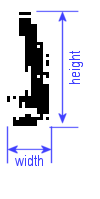
\includegraphics[width=0.1\textwidth]{inc/raster/design2-12.png}
  \caption{Пример цифры 1}
  \label{fig:fig212}
\end{figure}
Цифра один на ~\ref{fig:fig212} является частным случаем . Так как она похожа на 4 и 7, то метод определения, данный выше, может оказаться ненадёжным. Специфичный параметр единицы: в нашем случае, её ширина на 40\% меньше, чем высота. Нет другой такой цифры с таким же соотношением. У нас уже есть 25 зон (признаков), так вот это является 26-м признаком.

\begin{figure}[ht!]
  \centering
  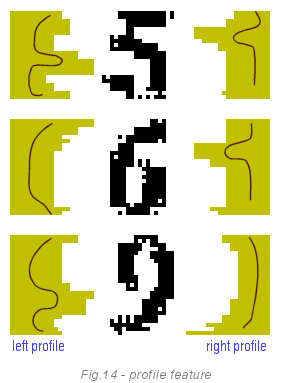
\includegraphics[width=0.5\textwidth]{inc/raster/design2-13.png}
  \caption{Пример цифры 1}
  \label{fig:fig212}
\end{figure}
Качество OCR может быть улучшено введением новых признаков. Например, цифры 5,6 и 9 очень похожи при использовании разбиения на зоны. Для того, чтобы различать их, мы можем использовать их профили как признаки. Особенностью признака является количество пикселей (расстояние) между краем рамки цифры и её границей.

На изображении ниже, вы можете видеть, что профили цифр 5 и 6 похожи, но они отличаются от профиля 9. Левый профиль 5 и 9 похож, но отличается от профиля 6.

\subsubsection{Корректировка результатов OCR}

Как только OCR закончен, результаты корректируются в соответствии с правилами судоку. 

В одной строке, столбце и блоке 3х3 не может находиться одна и та же цифра. Если правило нарушено, то необходимо ввести коррективы в полученные результаты. Мы заменим неправильную цифру той, что возможна из оставшихся. 

Например, на рис.~\ref{fig:fig211} выше, результат 5 потому что $diff = 5210$, которое является самым маленьким значением различия. Следующий возможный результат $6$, так как $diff = 5508$ в этом случае. Таким образом, мы заменим $5$ на $6$. Чтобы решить, которая из двух цифр неверная, мы сравним значения их различий с их образцами, и та, у которой значение меньше, будет считаться верной. 

\subsection{Принцип работы системы}
 Область распознавания изображений является одной из самых захватывающих в современных компьютерных вычислениях, и она очень сложна. Что легко и просто для человеческого мозга, то очень сложно для системы. Многие вещи до сих пор остаются невозможными с сегодняшним уровнем развития IT.

На блок-схеме на рис.~\ref{fig:fig211} представлены все этапы, которые проходит изображение перед тем, как будет распознано.
\begin{figure}[ht]
  \centering
  \includegraphics[width=0.3\textwidth]{inc/dia/design2-14}
  \caption{Блок-схема подсистемы распознавания}
  \label{fig:fig214}
\end{figure}

На рис.~\ref{fig:fig211} представлена диаграмма классов подсистемы распознавания.


\begin{figure}[ht]
  \centering
  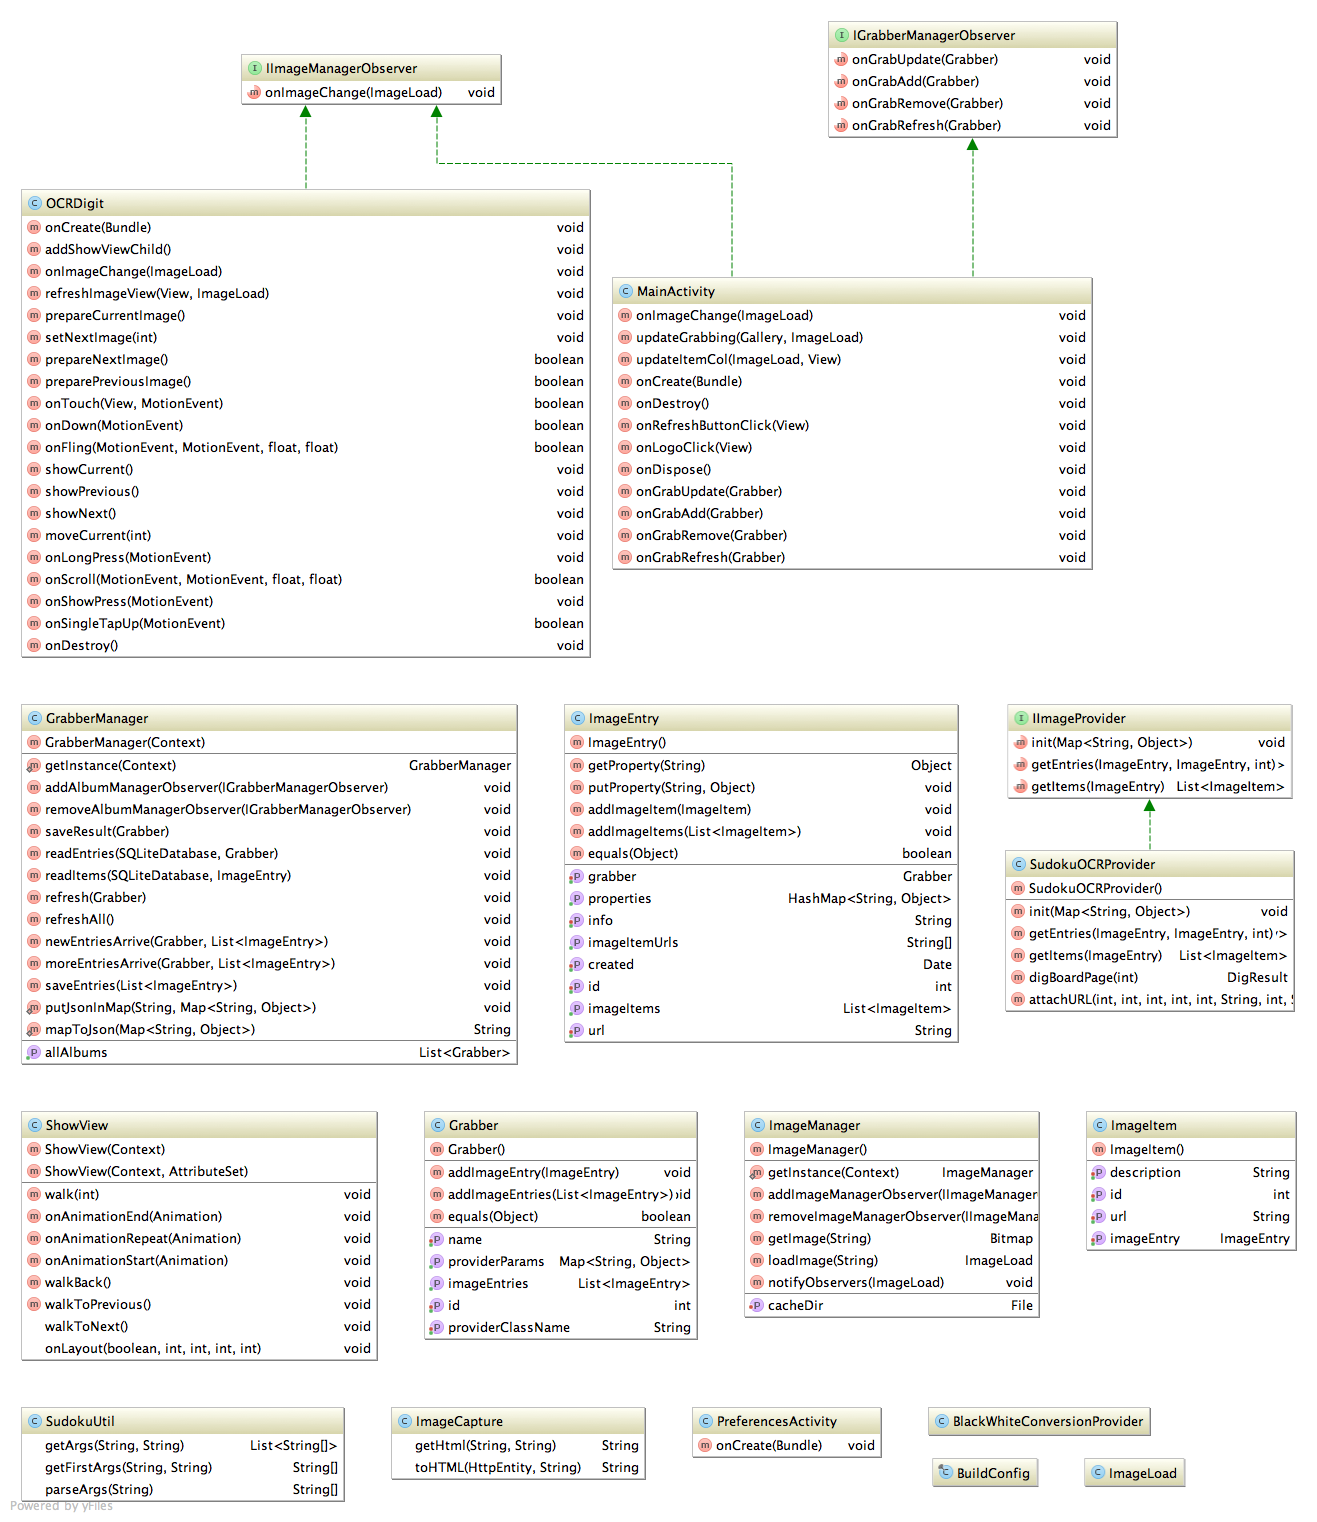
\includegraphics[width=\textwidth]{inc/raster/design2-15.png}
  \caption{Диаграмма классов OCR}
  \label{fig:fig2100}
\end{figure}

После распознавания мы сохраняем результаты в CSV-файл.

Для обмена данными между роботом и мобильным устройством будем использовать формат CSV.

\paragraph{CSV} (от англ. Comma-Separated Values — значения, разделённые запятыми) — текстовый формат, предназначенный для представления табличных данных. Каждая строка файла — это одна строка таблицы. Значения отдельных колонок разделяются разделительным символом (delimiter) — запятой (,). Однако, большинство программ вольно трактует стандарт CSV и допускают использование иных символов в качестве разделителя. 

Пример распознанного изображения в формате CSV:
\begin{lstlisting}[caption=CSV файл с задание]
5,3,,,7,,,,
6,,195,,
,9,8,,,,6,
8,,,6,,,,3
4,,8,,3,,1
7,,,2,,,6
,6,,,,,2,8,
,,,4,1,9,,,5
,,,,8,,,7,9
\end{lstlisting}

Нас данный вариант устраивает, так формат достаточно компактен для передачи и нам не нужно "захлямлять" информационным шумом потоки передачи данных. 

\section{Подсистема передачи данных}

Нашей наиболее часто выполняемой задаче будет передача распознанного CSV-файла с мобильного телефона на контроллер робота.

В листинге~\ref{lst:analyt1} и листинге~\ref{lst:analyt2} приведены примеры обмена данными между роботом и телефоном, описанные в протоколе сообщений робота.

Процесс сопряжения мы можем произвести с помощью встроенных возможностей каждого из устройств, поэтому дублировать его не имеет смысла и воспользуемся стандартной процедурой сопряжения.

\subsection{Обмен данными между устройствами}

У нас есть список команд, описание протокола, сформированный файл, но проблема в том, что у нас лимит сообщения 64 байта.

Нам неудобно разрывать файл, управляющие команды и остальные сообщения на большое количество частиц.

Для этого мы воспользуемся \textbf{Bluetooth сокетами}.

\paragraph{Bluetooth сокет} -  API, позволяющий реализовывать взаимодействие между компьютерами или между процессами на одном компьютере. Данная технология может работать со множеством различных устройств ввода-вывода и драйверов, несмотря на то, что их поддержка зависит от реализации операционной системы.

С мобильного устройства у нас будут отправляться данные, а на роботе будут приниматься.

На телефоне мы создаем отправляющий сокет, приведенный в листинге~\ref{lst:design1} 

\begin{lstlisting}[caption={Создаем сокет с данными для отправки}, label=lst:design1, language=Java]
Method m = device.getClass().getMethod("createRfcommSocket", new Class[] { int.class }); 
BluetoothSocket sendSocket = (BluetoothSocket) m.invoke(device, 1);
\end{lstlisting}

% \begin{lstlisting}[caption={Формат команд для получения потока данных}, label=lst:analyt1]
% MessageWrite

% Byte 0: 0x00 or 0x80
% Byte 3: Message size
% Byte 4: Message Text
% \end{lstlisting}











\chapter{Технологический раздел}
\label{cha:impl}

В данном разделе описываются используемые при работе над проектом инструменты и технологии.

\section{Выбор языка программирования}

Для реализации системы выбран язык Java. Перечислим основные преимущества, говорящие в пользу его использования.
Java является объектно-ориентированным языком. Это дает возможность при разработке приложений использовать технологию объектно-ориентированного программирования, которая позволяет сократить общее время разработки и писать повторно используемый код.

Java-приложения являются независимыми от платформы. Это достигается путем совмещения в языке свойств компилятора и интерпретатора следующим образом: классы программы компилируются во внутренний байт-код, который может интерпретирован виртуальной java-машиной (JVM, Java Virtual Machine). 

Платформонезависимость байт-кода обеспечивается наличием виртуальных java-машин для всех основных платформ.

В комплект поставки Java (JDK, Java Developer Kit) входят стандартные классы, которые обладают достаточной функциональностью для быстрой разработки приложений.

Важным преимуществом является наличие большого количества библиотек, расширяющих возможности языка.

\section{Используемые библиотеки и модули}
\subsection{Мобильное приложение}

\paragraph{Android} — операционная система для смартфонов, планшетных компьютеров, электронных книг, цифровых проигрывателей, наручных часов, игровых приставок, нетбуков, смартбуков, других устройств. Основана на ядре Linux и собственной реализации Java от Google. 

Android позволяет создавать Java-приложения, управляющие устройством через разработанные Google библиотеки. Android Native Development Kit позволяет портировать библиотеки и компоненты приложений.

\subsection{Android SDK}

Приложения под операционную систему Android являются программами в нестандартном байт-коде для виртуальной машины Dalvik, для них был разработан формат установочных пакетов .APK.

Google предлагает для свободного скачивания инструментарий для разработки (Software Development Kit), который предназначен для x86-машин под операционными системами Linux, Mac OS X (10.4.8 или выше), Windows XP, Windows Vista и Windows 7. Для разработки требуется JDK 5 или более новый.

Разработку приложений для Android можно вести на языке Java (не ниже Java 1.5).

Существует плагин для Eclipse — Android Development Tools (ADT), предназначенный для Eclipse версий 3.3—3.7. Также существует плагин для IntelliJ IDEA, облегчающий разработку Android-приложений, и для среды разработки NetBeans IDE, который, начиная с версии NetBeans 7.0, перестал быть экспериментальным, хоть пока и не является официальным.

Кроме того, существует Motodev Studio for Android — комплексная среда разработки на базе Eclipse, позволяющая работать непосредственно с Google SDK.

В целом, \textbf{Andoroid SDK} предоставляет нам все необходимые средства для реализации заявленных задач.

\subsection{ПО для контроллера робота}

\paragraph{leJOS} является заменой прошивки для программируемых блоков Lego Mindstorms.

В настоящее время она поддерживает LEGO RCX блок и Lejos NXJ поддерживает блок NXT. Она включает в себя виртуальную машину Java, что позволяет Lego Mindstorms роботам писать программное обеспечение на языке программирования Java. 

Так как Lejos NXJ является проектом Java, она основывается на богатстве функциональных возможностей, присущей платформе Java. Существуют Lejos NXJ плагины для двух ведущих IDE для Java: Eclipse и NetBeans. Разработчики могут воспользоваться стандартной функциональности в IDE (автозавершения кода, рефакторинга и шаблонов для тестирования), а также такие возможности как: компиляция, сборка и выгрузки. 

Lejos NXJ обеспечивает поддержку доступа к портам робота. Это позволяет получить доступ к стандартным датчикам и двигателям (ультразвуковой датчик расстояния, сенсорный датчик, звук и датчик света). Другие компании, такие как MindSensors и HiTechnic распространили этот базовый набор, предоставляя усовершенствованные датчики, исполнительные механизмы и мультиплексоры. Lejos NXJ включает Java API, для этих продуктов.

Воспользовавшись объектно-ориентированной структурой языка Java, разработчики Lejos NXJ смогли скрыть детали реализации датчиков. Это позволяет разработчику работать с абстракциями высокого уровня, не беспокоясь о деталях, например таких как шестнадцатеричная адресация аппаратных компонентов.

Проект включает в себя реализацию наиболее часто используемых контроллером обратной связи, ПИД-регулятора и алгоритма снижения фильтр шума Калмана. Lejos NXJ также предоставляет библиотеки, которые поддерживают более абстрактные функции, такие как навигации, картографирования и поведения.

\begin{lstlisting}[caption={Пример кода для работы с двигателями}, language=Java]
import lejos.nxt.Motor;
import lejos.nxt.Button;

public class Example {
    public static void main(String[] args) {
        Motor.A.forward();
        Button.waitForPress();
        Motor.A.backward();
        Button.waitForPress();
        System.exit(1);
    }
}
\end{lstlisting}


Таким образом, мы можем писать на удобном нам языке (в данном случае Java) и работать с подключаемыми устройствами робота посредством API, просто делая импорт нужной библиотеки, которая отвечает за управляющие команды или данные сенсоров.

\section{Система контроля версий}
\subsection{Git}

В качестве системы контроля версий была выбрана CVS Git. Данный инструмент является очень популярным и удобным в работе. Не требует установки сервера при одиночной разработке.

Работа с подмодулями в данной системе упрощает разработку и интеграцию нескольких проектов параллельно, что является большим плюсом в работе, поскольку каждый компонент системы был оформлен как отдельный репозиторий git.


\section{Среда разработки}
Выбор описанных выше инструментов привел к естественному выбору IDE, поддерживающей как язык Java и работу с его зависимостями и библиотеками, так и обладающей интеграцией с CVS Git. Такой средой стала программа IntelliJ IDEA компании JetBrains. 
\subsection{IntelliJ IDEA}

Данная среда разработки создана специально для разработки на языке Java и имеет отличные инструменты для отладки программ, запуска модульных и функциональных тестов с возможностью отображения покрытия кода тестами, эмулятор командой строки для быстрого запуска консольных команд, систему управления библиотеками Java, а так же поддержка всевозможных Java фреймворков и библиотек и всех его основных функций. 

Подсветка синтаксиса, автодополнение, инспекция кода и другие функции облегающие жизнь разработчика так же присутствуют в данной IDE, а прекрасное выполнения функции поиска классов и файлов проекта экономит значительное количество времени.

Так же кроме написания ПО на языке Java, IntelliJ IDEA поддерживает работу с другими языками, документами HTML, CSS-стилями и JavaScript-скриптами. Поддержка манифест-файлов для разного рода приложений, умение понимать, анлизировать и определять вставки исходного кода на другом языке облегчают процесс разработки.

Таким образом данная программа является идеальным решением для разработки на языке Java и в частности Java, Android и других производных приложений.

\section{База данных}
\subsection{SQLite}
\paragraph{SQLite} - компактная встраиваемая реляционная база данных. Исходный код библиотеки передан в общественное достояние.

Слово «встраиваемый» означает, что SQLite не использует парадигму клиент-сервер, то есть СУБД SQLite не является отдельно работающим процессом, с которым взаимодействует программа, а предоставляет библиотеку, с которой программа компонуется и СУБД становится составной частью программы. Таким образом, в качестве протокола обмена используются вызовы функций (API) библиотеки SQLite. Такой подход уменьшает накладные расходы, время отклика и упрощает программу.

SQLite хранит всю базу данных (включая определения, таблицы, индексы и данные) в единственном стандартном файле на том компьютере, на котором исполняется программа. Простота реализации достигается за счёт того, что перед началом исполнения транзакции записи весь файл, хранящий базу данных, блокируется; ACID-функции достигаются в том числе за счёт создания файла журнала.

Несколько процессов или потоков могут одновременно без каких-либо проблем читать данные из одной базы. Запись в базу можно осуществить только в том случае, если никаких других запросов в данный момент не обслуживается; в противном случае попытка записи оканчивается неудачей, и в программу возвращается код ошибки. Другим вариантом развития событий является автоматическое повторение попыток записи в течение заданного интервала времени.

В комплекте поставки идёт также функциональная клиентская часть в виде исполняемого файла sqlite3, с помощью которого демонстрируется реализация функций основной библиотеки. Клиентская часть работает из командной строки, позволяет обращаться к файлу БД на основе типовых функций ОС.

Благодаря архитектуре СУБД возможно использовать SQLite как на встраиваемых системах, так и на выделенных машинах с гигабайтными массивами данных.

Таким образом SQLite идеально подходит для реляционного хранения данных на мобильном устройстве под управлением ОС Android схема которой представлена на рис~\ref{fig:fig25}
\begin{figure}[ht!]
  \centering
  \includegraphics[width=\textwidth]{inc/dia/impl4-1}
  \caption{ER диаграмма}
  \label{fig:fig25}
\end{figure}



%%% Local Variables:
%%% mode: latex
%%% TeX-master: "rpz"
%%% End:

\chapter{Экспериментальный раздел}
\label{cha:research}



%%% Local Variables:
%%% mode: latex
%%% TeX-master: "rpz"
%%% End:


\chapter{Организационно-экономический раздел}

Организационно-экономическая часть процесса разработки программного продукта предусматривает выполнение следующих работ:
\begin{itemize}
\item формирование состава выполняемых работ и группировка их по стадиям разработки;
\item расчет трудоемкости выполнения работ;
\item установление профессионального состава и расчет количества исполнителей;
\item определение продолжительности выполнения отдельных этапов разработки;
\item построение календарного графика выполнения разработки;
\item контроль выполнения календарного графика.
\end{itemize}

\section{Формирование состава выполняемых работ и группировка их по стадиям разработки}

Разработку программного продукта можно разделить на следующие стадии:

\begin{itemize}
\item техническое задание;
\item расчет трудоемкости выполнения работ;
\item эскизный проект;
\item технический проект;
\item рабочий проект;
\item внедрение.
\end{itemize}

Допускается объединение технического и рабочего проекта в технорабочий проект.

Планирование длительности этапов и содержания проекта осуществляется в соответствии с ЕСПД ГОСТ 34.603--92 и распределяет работы по этапам. как показано в таблице \ref{tab:jobsAndStages}.

\newpage
\footnotesize
\begin{longtable}{|l|c|p{0.65\textwidth}|}
    \caption{Распределение работ проекта по этапам}
    \label{tab:jobsAndStages}
        \\ \hline
        \multicolumn{1}{|l|}{\centering Основные стадии}
      & \multicolumn{1}{|c|}{\centering \No}
      & \multicolumn{1}{|p{0.5\textwidth}|}{\centering Содержание  работы} \\
        \hline
            \endfirsthead
        
        \subcaption{\normalsize Продолжение таблицы~\ref{tab:jobsAndStages}}
        \\ \hline \endhead
        \subcaption{\normalsize Продолжение на следующей странице}
        \endfoot
        \hline
        \endlastfoot
        
        \multirow{2}{*}{\centering 1. Техническое задание} & 1 & Постановка задачи \\
        \cline{2-3}
        & 2 & Выбор средств проектирования и разработки \\
        \hline
        \multirow{4}{*}{\centering 2. Эскизный проект} & 3 & Разработка структуры системы \\
        \cline{2-3}
        & 4 & Разработка алгоритмов описания моделей и моделирования \\
        \cline{2-3}
        & 5 & Разработка вспомогательных алгоритмов \\
        \cline{2-3}
        & 6 & Разработка пользовательского интерфейся \\
        \hline
        \multirow{7}{*}{\centering 2. Технорабочий проект} & \centering 7 & Реализация алгоритмов описания моделей и моделирования\\
        \cline{2-3}
        & 8 & Реализация вспомогательных алгоритмов \\
        \cline{2-3}
        & 9 & Реализация пользовательского интерфейса \\
        \cline{2-3}
        & 10 & Отладка программного продукта \\
        \cline{2-3}
        & 11 & Исправление ошибок и недочетов \\
        \cline{2-3}
        & 12 & Разработка документации к системе \\
        \cline{2-3}
        & 13 & Итоговое тестирование системы \\
        \hline
        4. Внедрение & 14 & Установка и настройка программного продукта \\
        \hline
\end{longtable}
\normalsize

\section{Расчет трудоемкость выполнения работ}

Трудоемкость разработки программной продукции заывисит от ряда факторов, основными из которых являются следующие:

\begin{itemize}
\item степень новизны разрабатываемого программного продукта;
\item сложность алгоритма его функционирования;
\item объем используемой информации, вид ее представления и способ обработки;
\item уровень используемого алгоритмического языка программирования.
\end{itemize}

Разрабатываемый программный продукт можно отнести:

\begin{itemize}
\item по степени новизны~--- к категории В. Разрботка программной продукции имеющей аналоги. 
\item по степени сложности алгоритма функционирования~--- к 1-ой группе (программная продукиця реализующая моделирующие алгоритмы). 
\end{itemize}

Трудоемкость разработки программного продукта $\tau_{\text{ПП}}$ может быть определена как сумма величин трудоемкости выполнения отдельных стадий разработки ПП из выражения~\ref{F:tayPP}.

\begin{equation}
\tau_{\text{ПП}} = \tau_{\text{ТЗ}} + \tau_{\text{ЭП}} + \tau_{\text{ТП}} + \tau_{\text{РП}} + \tau_{\text{В}}
\label{F:tayPP}
\end{equation}, где

$\tau_{\text{ТЗ}}$~--- трудоемкость разработки технического задания; $\tau_{\text{ЭП}}$~--- трудоемкость разработки эскизного проекта; $\tau_{\text{ТП}}$~--- трудоемкость разработки технического проекта; $\tau_{\text{РП}}$~--- трудоемкость разработки рабочего проекта; $\tau_{\text{В}}$~--- трудоемкость внедрения.

Трудоемкость разработки технического задания рассчитывается по формуле~\ref{F:tayTZ}

\begin{equation}
\tau_{\text{ТЗ}} = T_{\text{ЗРЗ}} + T_{\text{ЗРП}}
\label{F:tayTZ}
\end{equation}, где

$T_{\text{ЗРЗ}}$~--- затраты времени разработчика постановки задач на разработку ТЗ, чел.-дни; $T_{\text{ЗРП}}$~--- затраты времени разработчика ПО на раззработку ТЗ, чел.-дни.

Значения величин $T_{\text{ЗРЗ}}$ и $T_{\text{ЗРЗ}}$ рассчитываются по формулам \ref{F:TZRZ} и \ref{F:TZRP}.

\begin{equation}
T_{\text{ЗРЗ}} = t_{\text{З}} \cdot K_{\text{ЗРЗ}}
\label{F:TZRZ}
\end{equation}

\begin{equation}
T_{\text{ЗРП}} = t_{\text{З}} \cdot K_{\text{ЗРП}}
\label{F:TZRP}
\end{equation}, где

$t_{\text{З}}$~--- норма времени на разработку ТЗ на ПП в зависимости от его функционального назначенияя и стпени новизны, чел.-дни; $K_{\text{ЗРЗ}}$~--- коэффициент, учитывающий удельный вес трудоемкости работ, выполняемых разработчикм ТЗ; $K_{\text{ЗРЗ}}$~--- коэффициент, учитывающий удельный вес трудоемкости работ, выполняемых разраьотчиком ПО на стадии ТЗ.

$t_{\text{З}} = 24$~чел.-дн. (управление НИР)

$K_{\text{ЗРЗ}} = 0.65$ (совместная разработка)

$K_{\text{ЗРП}} = 0.35$ (совместная разработка)

$\tau_{\text{ТЗ}} = 24 \cdot 0.65 + 24 \cdot 0.35 = 24$~чел.-дн.

Аналогично рассчитывается трудоемкость эскизного проекта $\tau_{\text{ЭП}}$:

$\tau_{\text{ЭП}} = 70 \cdot 0.5 + 70 \cdot 0.5 = 70$~чел.-дн.

Трудоемкость разработки технического проекта $\tau_{\text{ТП}}$ зависит от функционального назначения ПП, количества разновидностей форм входной и выходной информации и определяется как сумма времени, затраченного разрабьотчикм постановки задач и разработчиком программного обеспечения по формуле~\ref{F:tauTP}.

\begin{equation}
\tau_{\text{ТП}} = (t_{\text{ТРЗ}} + t_{\text{ТРП}}) \cdot K_{\text{В}} \cdot K_{\text{Р}}
\label{F:tauTP}
\end{equation}, где

$t_{\text{ТРЗ}}$ и $t_{\text{ТРП}}$~--- норма времени, затрачивваемого на разработку ТП разрабьотчиком постановки задач и разработчиком программного обуспечения соответственно, чел.-дни; $K_{\text{В}}$~--- коэффициент учета вида используемой информации, $K_{\text{Р}}$~--- коэффициент учета режима обработки информации.

Значение коэффициента $K_{\text{В}}$ определяется из выражения:

\begin{equation}
K_{\text{В}} = \frac{K_{\text{П}} \cdot n_{\text{П}} + K_{\text{НС}} \cdot n_{\text{НС} + K_{\text{Б}} \cdot n_{\text{Б}}}}{n_{\text{П}} + n_{\text{НС}} + n_{\text{Б}}}
\end{equation}

где  $K_{\text{П}}$, $K_{\text{НС}}$, $K_{\text{Б}}$~--- значения коэффициентов учета вида используемой информации для переменной, нормативно-справочной информации и баз данных соответственно; $n_{\text{П}}$, $n_{\text{НС}}$, $n_{\text{Б}}$~--- количество наборов данных переменной, нормативно-справочной информации и баз данных соответственно.

$K_{\text{П}} = 1$, $K_{\text{НС}}$ - 0.72, $K_{\text{Б} = 2.08}$

$K_{\text{В}} = \frac{1 \cdot 3 + 0.72 \cdot 1 + 2.08 \cdot 0}{3 + 1 + 0} = 0.505$

$K_{\text{Р}} = 1.26$

$\tau_{\text{ТП}} = (33 + 10) \cdot 0.505 \cdot 1.26 = 28$, чел.-дн.

Трудоемкость разработки рабочего проекта $\tau_{\text{РП}}$ зависит от функционального назначения ПП, количества разновидностей форм входной информации, сложности алгоритма функционирования, сложности контроля информации, степени использования готовых программных модулей, уровня алгоритмического языка программирования и определяется по формуле:

\begin{equation}
\tau_{\text{РП}} = K_{\text{К}} \cdot K_{\text{Р}} \cdot K_{\text{Я}} \cdot K_{\text{З}} \cdot K_{\text{ИА}} \cdot (t_{\text{РРЗ}} + t_{\text{РРП}})
\label{F:tauRP}
\end{equation}

где $K_{\text{К}}$~--- коэффициент учета сложности контроля информации; $K_{\text{Я}}$~--- коэффициент учета уровня используемого алгоритмического языка программирования; $K_{\text{З}}$~--- коэффициент учета степени использования готовых программных модулей; $K_{\text{ИА}}$~--- коэффициент учета вида используемой информации и сложности алгоритма ПП.

$K_{\text{К}} = 1, K_{\text{Р}} = 1.44, K_{\text{Я}} = 1, K_{\text{З}} = 0.7, t_{\text{РРЗ}} = 9$~чел.-дн., $t_{\text{РРП}} = 54$~чел.-дн., $K_{\text{П}} = 1.2, K_{\text{НС}} = 0.65, K_{\text{Б}} = 0.54$

$K_{\text{ИА}} = \frac{1.2 \cdot 3 + 0.65 \cdot 1 + 0.54 \cdot 0}{3 + 1 + 0} = 1.06$

$\tau_{\text{РП}} = 1 \cdot 1.44 \cdot 1 \cdot 0.7 \cdot 1.06 \cdot (9 + 54) = 67$

Так как при разработке ПП стадии <<Технический проект>> и <<Рабочий проект>> объеденины в стадию <<Техно-рабочий проект>>, то трудоемоксть ее выполнения $\tau_{\text{ТРП}}$ определяется по формуле:

\begin{equation}
\tau_{\text{ТРП}} = 0.85 \cdot (\tau_{\text{ТП}} + \tau_{\text{РП}})
\label{F:tauTRP}
\end{equation}
$\tau_{\text{ТРП}} = 0.85 \cdot (28 + 67) = 91$


Трудоемкость выполнения стадии внедрения $\tau_{\text{В}}$ может быть расчитана по формуле:

\begin{equation}
\tau_{\text{В} = (t_{\text{ВРЗ}} + t_{\text{ВРП}}) \cdot K_{\text{К}} \cdot K_{\text{Р}} \cdot K_{\text{З}}}
\label{F:tauV}
\end{equation}

где $t_{\text{ВРЗ}}$, $t_{\text{ВРП}}$~--- норма времени, затрачиваемого разработчиком постановки задач и разработчиком ПО соответственно на выполнение процедур внедрения ПП, чел.-дни.

$\tau_{\text{В}} = (10 + 11) \cdot 1 \cdot 1.26 \cdot 0.7 = 19$ чел.-дн.

Подставив полученные данные в формулу~\ref{F:tayPP} получим:

$\tau_{\text{ПП}} = 24 + 70 + 91 + 19 = 204$ чел.-дн.

\begin{table}[ht]\footnotesize
    \caption{Распределение трудоемкости по стадиям разработки проекта}
    \begin{tabular}{|c|c|c|p{0.70\textwidth}|c|}
    \hline
    \begin{sideways}Этап\end{sideways} &
    \begin{sideways} \parbox{30mm}{Трудоемкость \\этапа, чел.-дн. }\end{sideways} &
    \No & \multicolumn{1}{p{0.7\textwidth}|}{\centering Содержание работы}&
    \begin{sideways} \parbox{30mm}{Трудоемкость, чел.-дн. }\end{sideways} \\
    \hline
    \multirow{2}{*}{\centering 1} & \multirow{2}{*}{\centering 24} & 1 & Постановка задачи, разработка ТЗ & 20 \\
    \cline{3-5}
    & & 2 & Выбор средств проектирования и разработки & 4\\
    \hline
    \multirow{4}{*}{\centering 2} & \multirow{4}{*}{\centering 70} & 3 & Разработка структуры системы & 15 \\
    \cline{3-5}
    & & 4 & Разработка алгоритмов описания модели и моделирования & 30\\
    \cline{3-5}
    & & 5 & Разработка вспомогательных алгоритмов & 15\\
    \cline{3-5}
    & & 6 & Разработка пользовательского интерфейса & 10\\
    \hline
    \multirow{7}{*}{\centering 3} & \multirow{7}{*}{\centering 91} & 7 & Реализация алгоритмов описания модели и моделирования & 23 \\
    \cline{3-5}
    & & 8 & Реализация вспомогательных алгоритмов & 16\\
    \cline{3-5}
    & & 9 & Реализация пользовательского интерфейса & 10\\
    \cline{3-5}
    & & 10 & Отладка программного продукта & 12\\
    \cline{3-5}
    & & 11 & Исправление ошибок и недочетов & 15\\
    \cline{3-5}
    & & 12 & Разработка документации к системе & 8\\
    \cline{3-5}
    & & 13 & Итоговое тестирование системы & 7\\
    \hline
    4 & 19 & 14 & установка и настройка ПП & 19 \\
    \hline
    & & &{\raggedleft{Итого:}} & 204 \\
    \hline
    \end{tabular}
\end{table}

\normalsize

\section{Расчет количества исполнителей}

Средняя численность исполнителей при реализации проекта разработки и внедрения ПО определяется соотношением:

\begin{equation}
N = \frac{Q_{\text{Р}}}{F}
\label{F:N}
\end{equation}

где $Q_{\text{Р}}$~--- затраты труда на выполнение проекта (разработка и внедрение ПО); $F$~--- фонд рабочего времени.

Величина фонда рабочего времени определяется соотношением:

\begin{equation}
F = T \cdot F_M
\label{F:F}
\end{equation}

где $T$~--- фвремя выполнения проекта в месяцах, равное 4 месяцам; $F_M$~--- фонд времени в текущем месяце, который рассчитывается из учета числа дней в году, числа выходных и праздничных дней:

\begin{equation}
F_M = \frac{t_{\text{р}} \cdot (D_{\text{К}} - D_{\text{В}} - D_{\text{П}})}{12}
\label{F:FM}
\end{equation}

где $t_{\text{р}}$~--- продолжительность рабочего дня; $D_{\text{К}}$~--- общее число дней в году; $D_{\text{В}}$~--- число выходных дней в году; $D_{\text{П}}$~--- число праздничных дней в году.

$F_M = \frac{8 \cdot (365 - 103 - 10)}{12} = 168$

$F = 4 \cdot 168 = 672$

$N = \frac{204 \cdot 8}{672} = 3$~--- число исполнителей проекта.

\section{Календарный план-график}

\begin{table}[ht]\footnotesize
\caption{Планирование разработки}
\begin{tabular}{|p{0.2\textwidth}|l|p{0.25\textwidth}|p{0.17\textwidth}|l|}
\hline
Стадия разработки & Трудоемкость & Должность исполнителя& Распределение трудоемкости & Численность \\
\hline
\multirow{2}{0.2\textwidth}{Техническое задание} & \multirow{2}{*}{24} & Ведущий программист & 18(75\%) & 1\\
& & Программист 1 & 6(25\%) & 1 \\
\hline
\multirow{3}{0.2\textwidth}{Эскизный проект} & \multirow{3}{*}{70} & Ведущий программист & 26(37\%) & 1\\
& & Программист 1 & 27(39\%) & 1 \\
& & Программист 2 & 17(24\%) & 1 \\
\hline
\multirow{3}{0.2\textwidth}{Технорабочий проект} & \multirow{3}{*}{91} & Ведущий программист & 36(40\%) & 1\\
& & Программист 1 & 32(35\%) & 1 \\
& & Программист 2 & 23(25\%) & 1 \\
\hline
\multirow{2}{0.2\textwidth}{Внедрение} & \multirow{3}{*}{19} & Ведущий программист & 8(42\%) & 1\\
& & Программист 2 & 11(58\%) & 1 \\
\hline
\end{tabular}
\end{table}
\normalsize

\begin{table}[ht]\footnotesize
\caption{Календарный ленточный график работ}
\begin{tabular}{|l|l|llll|llll|llll|llll|}
\hline
Стадия разработки & Должность исполнителя & \multicolumn{16}{c|}{Трудоемкость} \\ 
\hline
\multirow{2}{0.2\textwidth}{Техническое задание} & Ведущий программист & \multicolumn{4}{l|}{\cellcolor[gray]{0.6}18} & & & & & & & & & & & &\\
& Программист 1 & \multicolumn{2}{l|}{\cellcolor[gray]{0.8}6} & {} & {} & & & & & & & & & & & & \\
\hline
\multirow{3}{0.2\textwidth}{Эскизный проект} & Ведущий программист & & & & & \multicolumn{4}{l|}{\cellcolor[gray]{0.8}26} & & & & & & & & \\
& Программист 1 & & & & & \multicolumn{4}{l|}{\cellcolor[gray]{0.6}27} & & & & & & & &\\
& Программист 2 & & & & &  \cellcolor[gray]{0.8}7 & {} & {} & \cellcolor[gray]{0.8}7 & & & & & & & & \\
\hline
\multirow{3}{0.2\textwidth}{Технорабочий проект} & Ведущий программист & & & & & & & & &\multicolumn{4}{l|}{\cellcolor[gray]{0.6}36} & & & & \\
& Программист 1 & & & & & & & & &\multicolumn{4}{l|}{\cellcolor[gray]{0.8}32} & & & & \\
& Программист 2 & & & & & & & & & {} & \multicolumn{3}{l|}{\cellcolor[gray]{0.8}23} & {} & & & \\
\hline
\multirow{2}{0.2\textwidth}{Внедрение} & Ведущий программист & & & & & & & & & & & & &\multicolumn{4}{l|}{\cellcolor[gray]{0.8}9} \\
& Программист 1 & & & & & & & & & & & & & \multicolumn{4}{l|}{\cellcolor[gray]{0.6}10}\\
\hline
\end{tabular}
\label{tab:timeline}
\end{table}

\normalsize 

Из таблицы~\ref{tab:timeline} видно, что благодаря параллельной работе ведущего программиста и программистов можно добиться сокращения сроков разработки с  204 дней до $18 + 27  + 36 + 11 = 92$ дней, т.е. в 2.2 раза.

\section{Расчет затрат на разработку ПП}

Затраты на выполнение проекта сосстоят из затрат на заработную плату исполнителям, затрат на закупку или аренду оборудования, затрат на организацию рабочих мест и затрат на накладные расходы. В таблице~\ref{tab:zarp} приведены затраты на заработную плату и страховые взносы во внебюджетные фонды. Суммарно эти отчисления для органиаций, осуществляющих деятельность в области информационных технологий, составляют 14\%: в Пенсионный фонд (ПФ)~--- 8\%, в Фонд социального стразования (ФСС), Федеральный и территориальный фонды обязательного медицинского страхования (ФФОМС и ТФОМС)~--- по 2\%. Для ведущего программиста предполагается ставка 2500 рублей за полный рабочий день, для первого программиста~--- 1500 рублей, для второго~--- 1000 рублей. 

\begin{table}[ht!]\footnotesize
\caption{Затраты на зарплату и отчисления во внебюджетные фонды}
\begin{tabular}{|l|l|l|l|l|l|l|}
\hline
& \multicolumn{6}{c|}{Февраль}\\
\hline
Исполниель & Рабочих дней & Зарплата & ПФ & ФСС & ФФОМС & ТФОМС\\
\hline
Ведущий программист & 20 & 50000 & 4000 & 1000 & 1000 & 1000\\
\hline
Программист 1 & 20 & 30000 & 2400 & 600 & 600 & 600\\
\hline
Программист 2 & 19 & 19000 & 1520 & 380 & 380 & 380\\
\hline
Итого: & \multicolumn{6}{r|}{112860}\\
\hline
& \multicolumn{6}{c|}{Март}\\
\hline
Исполниель & Рабочих дней & Зарплата & ПФ & ФСС & ФФОМС & ТФОМС\\
\hline
Ведущий программист & 22 & 55000 & 4400 & 1100 & 1100 & 1100\\
\hline
Программист 1 & 22 & 33000 & 2640 & 660 & 660 & 660\\
\hline
Программист 2 & 6 & 6000 & 480 & 120 & 120 & 120\\
\hline
Итого: & \multicolumn{6}{r|}{107160}\\
\hline
& \multicolumn{6}{c|}{Апрель}\\
\hline
Исполниель & Рабочих дней & Зарплата & ПФ & ФСС & ФФОМС & ТФОМС\\
\hline
Ведущий программист & 21 & 52500 & 4200 & 1050 & 1050 & 1050\\
\hline
Программист 1 & 21 & 31500 & 2520 & 630 & 630 & 630\\
\hline
Программист 2 & 10 & 10000 & 800 & 200 & 200 & 200\\
\hline
Итого: & \multicolumn{6}{r|}{107160}\\
\hline
& \multicolumn{6}{c|}{Май}\\
\hline
Исполниель & Рабочих дней & Зарплата & ПФ & ФСС & ФФОМС & ТФОМС\\
\hline
Ведущий программист & 20 & 50000 & 4000 & 1000 & 1000 & 1000\\
\hline
Программист 1 & 20 & 30000 & 2400 & 600 & 600 & 600\\
\hline
Программист 2 & 19 & 19000 & 1520 & 380 & 380 & 380\\
\hline
Итого: & \multicolumn{6}{r|}{112860}\\
\hline
& \multicolumn{6}{c|}{Июнь}\\
\hline
Исполниель & Рабочих дней & Зарплата & ПФ & ФСС & ФФОМС & ТФОМС\\
\hline
Ведущий программист & 16 & 40000 & 3200 & 800 & 800 & 800\\
\hline
Программист 1 & 15 & 22500 & 1800 & 450 & 450 & 450\\
\hline
Программист 2 & 3 & 3000 & 240 & 60 & 60 & 60\\
\hline
Итого: & \multicolumn{6}{r|}{74670}\\
\hline
Общая сумма: & \multicolumn{6}{r|}{446310}\\
\hline
\end{tabular}
\label{tab:zarp}
\end{table}
\normalsize

Расходы на материалы, необходимые для разработки ПП указаны в таблице~\ref{tab:materials}.

\begin{table}[ht!]\footnotesize
\caption{Материальные затраты}
\begin{tabular}{|c|p{0.25\textwidth}|l|c|c|c|}
\hline
\No & Наименование материала & Единица измерения & Кол-во & Цена за единицу, руб. & Сумма, руб.\\
\hline
1 & Бумага А4 & Пачка 500 л. & 1 & 150 & 150 \\
\hline
2 & Картридж для лазерного принтера Brother HL-2030R & Шт. & 2 & 1400 & 2800 \\
\hline
\multicolumn{5}{|r|}{Итого:} & 2950 \\
\hline
\end{tabular}
\label{tab:materials}
\end{table}

При разработке понадобится 3 компьютера (по одному на человека), один принтер, компьютерная мебель (3 комплекта), аксесуары для компьютеров (3 компьютера). Стоимость одной ПЭВМ составляет 35000 рублей. Месячная норма амортизации $K = 4\%$ (Срок службы~--- 25 месяцев). Срок службы составляет 3 года, месячная амортизация $K = 2.78\%$. Срок службы компьютерной мебели: столы~--- 5 лет, стулья~--- 2 года, месячные нормы амортизации~--- $K = 1.67\%$ и $K = 4.17\%$ соответственно. компьютерные аксесуары имеют срок службы 2 года, норма амортизации $K = 4.17\%$.

Затраты на амортизацию приведены в таблице~\ref{tab:amort}

\begin{table}[ht]\footnotesize
\caption{Амортизационные отчисления}
\begin{tabular}{|l|c|c|c|c|c|}
\hline
\parbox{20mm}{Наименование \\ оборудования} & \parbox{20mm}{Балансовая\\цена, руб.} & Кол-во, шт. & К, \% & {Время использования, мес.} & {Сумма отчислений, руб.} \\
\hline
Компьютер & 35000 & 3 & 4 & 4 & 16800 \\
\hline
Принтер & 2600 & 1 & 2.78 & 4 & 290 \\
\hline
Стол & 3000 & 3 & 1.67 & 4 & 600 \\
\hline
Стул & 1000 & 3 & 4.17 & 4 & 500 \\
\hline
Клавиатура & 500 & 3 & 4.17 & 4 & 350 \\
\hline
Мышь & 500 & 3 & 4.17 & 4 & 350 \\
\hline
\multicolumn{5}{|r|}{Итого:} & 18790 \\
\hline
\end{tabular}
\label{tab:amort}
\end{table}
\normalsize

Таке необходимо учесть аренднуюю полату за помещение, которая составляет 14000 рублей за месяц. За 4 месяца на аренду помещения уйдет 56000 рублей.

Общие затраты на разработку ПП составят $446310 + 2950 + 18790 + 56000 = 524050$ рублей.

\section{Расчет экономической эффективности}

Основными показателями экономической эффективности является чистый дисконтированный доход (ЧДД) и сок окупаемости вложенных средств.

Чистый дисконтированный доход определяется по формуле:

\begin{equation}
\text{ЧДД} = \sum_{t=0}^{T}{R_t - \text{З}_t \cdot \frac{1}{(1 + E)^t}}
\label{F:ChDD}
\end{equation}

где $T$~--- горизонт рачета по месяцам; $t$~--- период расчета; $R_t$~--- результат достигнутый на шаге (стоимость)$t$; $\text{З}_t$~--- затраты; $E$~--- приемлимая для инвестора норма прибыли на вложенный капитал.

Коэффициент $E$ установим равным ставке рефинансирования ЦБ РФ~--- 8\% годовых (0.67\% в месяц). В результате анализа рынка программной продукции, аналогичной разрабатваемой, планируется продажа 2 единц в 1-й месяц и 3 единицы в остальные. Планируемая цена ПП составляет 60000 рублей. Предполагаемые накладные расходы, связанные с реализацией составят 2000 рублей в месяц.

В таблице~\ref{tab:ChDD} приведен расчет ЧДД по месяцам работы над проектом, а на Рисунке~\ref{fig:ChDD} изображен график ЧДД (начерчен до момента, когда ЧДД принимает положительные значения).

\begin{table}[ht]\footnotesize
\caption{Расчет ЧДД}
\begin{tabular}{|c|c|c|c|c|c|}
\hline
Месяц & \parbox{20mm}{Текущие затраты, руб.}& \parbox{30mm}{Затраты с начала \\года, руб.}&\parbox{20mm} {Текущий \\доход, руб.}& \parbox{30mm}{Доход с начала\\года, руб.}& ЧДД, руб.\\
\hline
1 & 66451 & 66451 & 0 & 0 &-66451\\
\hline
2 & 126201 & 192652 & 0 & 0 &-192652\\
\hline 
3 & 126201 & 318853 & 0 & 0 &-318853\\
\hline
4 & 131901 & 450754 & 0 & 0 & -450754\\
\hline
5 & 73296 & 524050 & 60000 & 60000 &-464050\\
\hline
6 & 2000 & 526050 & 180000 & 240000 & -286050\\
\hline
7 & 2000 & 528050 & 180000 & 420000 & -108050\\
\hline
7 & 2000 & 530050 & 180000 & 600000 & 69950\\
\hline
\end{tabular}
\label{tab:ChDD}
\end{table}
\normalsize

 Срок окупаемости проекта~--- 8 месяцев.
 
\begin{figure}[ht]
 \centering
 \begin{tikzpicture}
    % \begin{axis}[
    %  width = 11cm,
    %  xlabel = {Время, мес.},
    %  ylabel = {ЧДД, руб.},
    %  xtick align = center,
    %  yminorgrids, ymajorgrids,
    %  xmajorgrids,
    %  minor y tick num = 4,
    %  legend style={at={(0.74,0.74)}, anchor=southwest}
    % ],
    % \addplot[black!80!black, mark=o, smooth] plot coordinates {
    %     (1,-66451)
    %     (2,-192652)
    %     (3,-318853)
    %     (4,-450754)
    %     (5,-464050)
    %     (6,-286050)
    %     (7,-108050)
    %     (8,69950)
    % };
    % \end{axis}
 \end{tikzpicture}
 \caption{График изменения ЧДД}
 \label{fig:ChDD}
\end{figure}


\section{Выводы}

По результатам расчета трудоемкости выполнения работ, затрат на выполнение работ и прибыли от реализации программного продукта был найден чистый дисконтированный доход по месяцам разработки и реализации программного продукта. На основе полученных данных можно сделать вывод, что проект эффективен и срок его окупаемости составляет 8 месяцев с начала разработки.
\chapter{Охрана труда и экология}

\section{Оценка условий труда на рабочем месте пользователя ПЭВМ}

Разработка ПО требует длительного взаимодействия с вычислительными системами. Работа с ПЭВМ связана с рядом вредных и опасных факторов, таких как статическое электричество, рентгеновское излучение, электромагнитные поля, блики отраженный свет, ультрафиолетовое излучение. При длительном воздействии на организм эти факторы негативно влияют на здоровье человека.

\subsection{Требования к организации рабочих мест}
При организации рабочего места должны учитываться следующие требования:
\begin{itemize}
\item достаточное рабочее пространство, позволяющее человеку осуществлять необходимые движения и перемещения при эксплуатации и техническом обслуживании;

\item оптимальное размещение оборудования;
\item необходимое естественное и искусственное освещение;
\item наличие необходимых средств защиты работающего персонала от действия вредных и опасных производственных факторов.
\end{itemize}

Важную роль играет планировка рабочего места, которая должна способствовать удобству выполнения работ, экономии электроэнергии и времени оператора, удобству обслуживания ЭВМ и отвечать правилам охраны труда.
В соответствии с ГОСТ Р 50923-96 «Дисплеи. Рабочее место оператора. Общие эргономические требования к производственной среде. Методы измерения» к организации рабочих мест предъявляются следующие ниже требования.
Экран видеомонитора должен находиться от глаз пользователя на расстоянии 600-700 мм, но не ближе 500 мм с учетом размеров алфавитно-цифровых знаков и сим- волов. Конструкция рабочего стола должна обеспечивать оптимальное размещение на рабочей поверхности используемого оборудования с учетом его количества и конструктивных особенностей, характера выполняемой работы. При этом допускается использование рабочих столов различных конструкций, отвечающих современным требованиям эргономики. Поверхность рабочего стола должна иметь коэффициент отражения 0,5-0,7. Регулируемая высота рабочей поверхности должна изменяться в пределах от 680 до 800 мм. Механизмы для регулирования высоты рабочей поверхности стола должны быть легко досягаемы в положении сидя, иметь простое управление и надежную фиксацию. Высота рабочей поверхности при нерегулируемой высоте должна составлять 725 мм. Поверхность рабочего стола должна иметь коэффициент отражения 0,5 - 0,7. Рабочая поверхность стола должна иметь следующие размеры: глубина не менее 600 мм; ширина не менее 1200 мм.

Рабочая поверхность стола не должна иметь острых углов и краев. Конструкция рабочего стула (кресла) должна обеспечивать поддержание рациональной рабочей позы при работе на ПЭВМ позволять изменять позу с целью снижения статического напряжения мышц шейно-плечевой области и спины для предупреждения развития утомления. Тип рабочего стула (кресла) следует выбирать с учетом роста пользователя, характера и продолжительности работы с ПЭВМ.
Рабочий стул (кресло) должен быть подъемно-поворотным, регулируемым по высоте и углам наклона сиденья и спинки, а также расстоянию спинки от переднего края сиденья, при этом регулировка каждого параметра должна быть независимой, легко осуществляемой и иметь надежную фиксацию. Поверхность сиденья, спинки и других элементов стула (кресла) должна быть полумягкой, с нескользящим, слабо электризующимся и воздухопроницаемым покрытием, обеспечивающим легкую очистку от загрязнений.
При размещении рабочих мест с ПЭВМ расстояние между рабочими столами с видеомониторами (в направлении тыла поверхности одного видеомонитора и экрана другого видеомонитора), должно быть не менее 2,0 м, а расстояние между боковыми поверхностями видеомониторов - не менее 1,2 м.

\subsection{Параметры микроклимата}

Параметры микроклимата могут меняться в широких пределах, в то время как необходимым условием жизнедеятельности человека является поддержание постоянства температуры тела благодаря терморегуляции, т.е. способности организма регулировать отдачу тепла в окружающую среду. Принцип нормирования микроклимата - создание оптимальных условий для теплообмена
тела человека с окружающей  средой. Вычислительная техника является источником существенных тепловыделений, что может привести к повышению температуры и снижению относительной влажности в помещении. В помещениях, где установлены компьютеры, должны соблюдаться определенные параметры микроклимата. Нормы, установленные СанПиН 2.2.2/2.4.1340-03 для категории работ 1а приведены в таблице~\ref{tab:microclimate}. Эти нормы устанавливаются в зависимости от времени года, характера трудового процесса и характера производственного помещения.

\begin{table}[ht]
\caption{Параметры микроклимата}
\begin{tabular}{|l|c|c|c|c|c|c|}
\hline
\multirow{2}{*}{Период год} & \multicolumn{2}{l|}{Температура, $^\circ \mbox{C}$} & \multicolumn{2}{l|}{Влажность, \%} & \multicolumn{2}{l|}{Скорость воздуха, м/с} \\
\cline{2-7}
&Оптим.&Допуст.&Оптим.&Допуст.&Оптим.&Допуст.\\
\hline
Холодный &22--24&21--25&40--60&75&0.1&0.1\\
\hline
Теплый &23--25&22--28&40--60&55 при 28$^\circ \mbox{C}$&0.1&0.1\\
\hline 
\end{tabular}
\label{tab:microclimate}
\end{table}

Вредным фактором при работе с ЭВМ является также запыленность помещения. Этот фактор усугубляется влиянием на частицы пыли электростатических полей персональных компьютеров.

Для устранения несоответствия параметров указанным нормам проектом предусмотренно использование системы кондиционирования как наиболее эффективного и автоматически функционирующего средства.

Нормы установленные содержания в воздухе положительных и отрицательной ионов, установленные СанПиН 2.2.4.1294--03, приведены в таблице~\ref{tab:ions}.

\begin{table}[ht]
\caption{Уровни ионизации воздуха при работе на ПЭВМ}
\begin{tabular}{|l|c|c|}
\hline
\multirow{2}{*}{Уровни} & \multicolumn{2}{l|}{Число ионов в кубометре воздуха}\\
\cline{2-3}
&$n^+$&$n^-$\\
\hline
Минимально необходимое & 400 & 600 \\
\hline
Оптимальное & 1500--3000 & 3000--5000 \\
\hline
Максимально допустимое & 50000 & 50000 \\
\hline
\end{tabular}
\label{tab:ions}
\end{table}

Для обеспечения требуемых уровней предусмотренно использование системы ионизации Сапфир-4А.

Объем помещений, в которых размещены работники вычислительных центров, не должен быть меньше $19.5 \frac{\text{м}^3}{\text{человека}}$ с учетом максимального числа одновременно работающих в смену. Нормы подачи свежего воздуха в помещения, где расположены компьютеры, приведены в таблице~\ref{tab:air}.

\begin{table}[ht]
\caption{Уровни ионизации воздуха при работе на ПЭВМ}
	\begin{tabular}{|l|l|}
	\hline
	Уровни & Число ионов в кубометре воздуха \\ 
	\hline
	Объем до $20 {\text{м}^3}$ на человека & Не менее 30 \\
	\hline
	$20.40 {\text{м}^3}$ на человека & Не менее 20 \\
	\hline
	Более $40 {\text{м}^3}$ на человека & Естественная вентиляция \\
	\hline
	\end{tabular}
\label{tab:air}
\end{table}

Для обеспечения комфортных условий используются как организационные методы (рациональная организация проведения работ в зависимости от времени года и суток, чередование труда и отдыха), так и технические средства (вентиляция, кондиционирование воздуха, отопительная система).

\subsection{Шум и вибрации}

Уровень шума на рабочем месте программиста не должен превышать 50 дБА, а уровень вибрации не должен превышать норм установленных СанПиН 2.2.2.542--96 (см. таблицу~\ref{tab:vibro}).

\begin{table}[ht]
\caption{Допустимые нормы вибрации на раочих местах с ПЭВМ}
\begin{tabular}{|c|c|c|}
\hline
\parbox{0.4\textwidth}{ Среднегеометрические частоты\\октавных полос, Гц}& \multicolumn{2}{l|}{Допустимые значения по виброскорости}\\
\cline{2-3}
&м/c &дБ\\
\hline
2  & $4.5\times10$ & 79 \\
\hline
4  & $2.2\times10$ & 73 \\
\hline
8  & $1.1\times10$ & 67 \\
\hline
16  & $1.1\times10$ & 67 \\
\hline
31.5 & $1.1\times10$ & 67 \\
\hline
63  & $1.1\times10$ & 67 \\
\hline
\parbox{0.4\textwidth}{ Корректированные значения\\и их уровни в дБ}& $2.0\times10$ & 72\\
\hline
\end{tabular}
\label{tab:vibro}
\end{table}

При разработке ПО внутренними источниками шума являются вентиляторы, а также принтеры и другие перефферийные устройства ЭВМ. Внешние источники шума~--- прежде всего, шум с улицы и из соседних помещений. Постоянные внешние источники шума, превышающего нормы, отсутствуют.

Для устранения превышения нормы проектом предусмотрено применение звукопоглощающих материалов для облицовки стен и потолка помещения, в котором осуществляется работа с вычислительной техникой.

\subsection{Освещение}

Наиболее важным условием эффективной работы программистов и пользователей является соблюдение оптимальных параметров системы освещения в рабочих помещениях.

Естественное освещение осуществляется через светопроемы, ориентированные в основном на север и северо-восток (для исключения попадания прямых солнечных лучей на экраны компьютеров) и обеспечивает коэффициент естественной освещенности (КЕО) не ниже 1.5\%.

В качестве искусственного освещения проектом предусмотрено использование системы общего освещения. в соответствии с СанПин 2.2.2/2.4.1340--03 освещенность на поверхности рабочего стола должна находиться в пределах 300--500 лк. Разрешается использование светильников местного освещения для работы в документами (при этом светильники не должны создавать блики на поверхности экрана).

Правильное расположение рабочих мест относительно источников освещения, отсутствие зеркальных поверхностей и использование матовых материалов ограничивает прямую (от источников освещения) и отраженную (от рабочих поверхностей) блескость. При  этом яркость светящихся поверхностей не превышает $200 \frac{\text{кд}}{\text{м}^2}$, яркость бликов на экране ПЭВМ не превышает $40 \frac{\text{кд}}{\text{м}^2}$, и яркость потолка не превышает $200 \frac{\text{кд}}{\text{м}^2}$.

В соответствии с СанПинН 2.2.2/2.4.1340--03 проектом предусмотрено использование люминесцентных ламп типа ЛБ в качестве источников света при искусственном освещении. В светильниках допускается применение ламп накаливания. Применение газоразрядных ламп в светильниках общего и местного освещения обеспечивает коэффициент пульсации не более 5\%.

Таким образом, проектом обеспечиваются оптимальные условия освещения рабочего помещения.

\subsection{Рентгеновское излучение}

В соответствии с СанПиН 2.2.2/2.4.1340-03 проектом предусмотрено использование ПЭВМ, конструкция которого обеспечивает мощность экспозиционной дозы рентгеновского излучения в любой точке на расстоянии 0.5 м. от экрана и корпуса не более 0.1 мбэр/час (100 мкР/час). Результаты сравнения норм излучения приведены в таблице~\ref{tab:rentgen}.

\begin{table}[ht]
\caption{Сравнение норм рентгеновского излучения в различных стандартах}
\begin{tabular}{|l|c|}
\hline
& Допустимое значение мкР/час, не более \\
\hline
СанПиН 2.2.2/2.4.1340-03 & 100 \\
\hline
ТСО-99 & 500 \\
\hline
MPR II & 500\\
\hline
\end{tabular}
\label{tab:rentgen}
\end{table}

Как видно из таблицы, стандарты MPR II и ТСО--99 предъявляют менее жесткие требования к рентгеновскому излучению, чем СанПиН. Но при соблюдении оптимального расстояния между пользователем и монитором дозы рентгеновского излучения не опасны для большинства людей.

\subsection{Неионизирующие электромагнитные излучения}

Допустимые значения параметров неионизирующих излучений в соответствии с СанПин 2.2.2/2.4.1340-03 приведены в таблицах~\ref{tab:U} и~\ref{tab:ro}.

\begin{table}[ht]
\caption{Предельно допустимые значения напряженности электрического поля}
\begin{tabular}{|c|c|}
\hline
Диапазон частот& Допустимые значения \\
\hline
5 Гц -- 2 кГц & 25 В/м \\
\hline
2 -- 400 кГц& 2.5 В/м \\
\hline
\end{tabular}
\label{tab:U}
\end{table}

\begin{table}[ht]
\caption{Предельно допустимые значения плотности магнитного потока}
\begin{tabular}{|c|c|}
\hline
Диапазон частот& Допустимые значения \\
\hline
5 Гц -- 2 кГц & 250 нТл \\
\hline
2 -- 400 кГц& 5 нТл \\
\hline
\end{tabular}
\label{tab:ro}
\end{table}

Величина поверхностного электрического потенциала не должна превышать 500 В.

Мониторы, используемые в настоящее время, удовлетворяют более жестким нормам MPR II, а значит и СанПиН.

\subsection{Визуальные параметры}

Неправильный выбор визуальных эргономических параметров приводит к ухудшению здоровья пользователей, быстрой утомляемости, раздражительности. В связи с этим, проектом предусмотрено, что конструкция вычислительной системы и ее эргономические параметры обеспечивают комфортное и надежное считывание информации. Требования к визуальным параметрам, их внешнему виду, дизайну, возможности настройки представлены в СанПиН 2.2.2/2.4.1340--03. Визуальные эргономические параметры монитора и пределы из изменений приведены в таблице~\ref{ergonom}.

\begin{table}[ht]
\caption{Визуальные эргономические параметры ВДТ и пределы из изменений}
\begin{tabular}{|l|c|c|}
\hline
\multirow{2}{*}{Наименование параметров} & \multicolumn{2}{c|}{Пределы значений параметров}\\
\cline{2-3}
&не менее&не более\\
\hline
Яркость экрана (фона), $\frac{\text{кд}}{\text{м}^2}$ (измеренная в темноте) &35&120\\
\hline
Внешняя освещенность экрана, лк &100&250\\
\hline
Угловой размер экрана, угл.мин. &16&60\\
\hline
\end{tabular}
\label{tab:ergonom}
\end{table}

Для выполнения этих требований проектом предусмотренно использование современных мониторов, имеющих достаточно широкий набор регулируемых параметров.  В частности, для удобного считывания информации реализована возможность настройки положения монитора по горизонтали и вертикали. Мониторы оснащены специальными устройствами и средствами настройки ширины, высоты, яркости, контраста и разрешения изображения. кроме того, в современных мониторах зерно изображения имеет размер в пределах 0.27 мм, что обеспечивает высокую четкость и непрерывность изображения. Наконец, на поверхность дисплея нанесено матовое покрытие, чтобы избавиться от солнечных бликов.

\section{Расчет искусственного освещения}

При расчете освещенности от светильников общего равномерного освещения наиболее часто применяют метод расчета по световому потоку. При расчете освещения по этому методу необходимое количество светильников для освещения рабочего места рассчитывается по формуле:

\begin{equation}
\label{f:lightsCount}
N = \frac{E_{min}\cdot S\cdot K}{F_\text{Л} \cdot \text{З} \cdot z \cdot h}
\end{equation}

где $E_{min}$~--- нормируемая минимальная освещенность; $S$~--- площадь помещения, $\text{м}^2$; $F_\text{Л}$~--- световой поток лампы, лк; $K$~--- коэффициент запаса; $z$~--- коэффициент неравномерности освещения (для люминесцентных ламп~---1.1); $h$~--- коэффициент использования светового потока в долях единицы.

$E_{min}$ определяется на основании нормативного документа СНиП23--05--95. В соответствии с произведенным выбором в предыдущем разделе, для работы программиста $E_{min}=300$ лк (общее освещение).

Работы, производятся в помещении, требуют различения цветных объектов при невысоких требованиях к цветоразличению, поэтому в качестве источника освещения была выбрана лампа люминесцентная холодно-белая (ЛХБ), 1940 лк, 30 Вт. В помещениях общественных и жилых зданий с нормальными условиями среды: К=1.4.

Для люминесцентных ламп коэффициент неравномерности освещения Z=1.1.

Коэффициент использования h зависит от типа светильника, от коэффициентов отражения потолка $\rho_\text{П}$, стен $\rho_\text{С}$, расчетной поверхности $\rho_\text{Р}$ и индекса помещения.

Высота подвеса над рабочей поверхностью Нр=3 м. Размеры помещения А=3.5 м, В=3 м. Определим индекс помещения по формуле:

\begin{equation}
\phi = \frac{A \cdot B}{H_P \cdot (A + B)} = \frac{3.5 \cdot 3}{s \cdot (3.5 + 3)} = 0.54
\end{equation}

Для светлого фона примем:$\rho_\text{П} = 70$ $\rho_\text{С} = 50$ $\rho_\text{Р} = 10$. h = 59\%.

Освещение проектируется при помощи светильников ОДОР с минимальной освещенностью $E_{min}=300$ лк, P=40 Вт. Число ламп в ОДОР равно 2. Необходимое число светильников для данной комнаты:

\begin{equation}
N = \frac{300 \cdot 9 \cdot 1.4}{1940 \cdot 0.59 \cdot 1.1 \cdot 2} = 2 \text{шт}
\end{equation}

Общее количество ламп $n = 2\times2=4$ шт. Длина светильника ОДОР=1.26 м. Поскольку длина помещения 3 м, то светильники помещаются в два ряда. 
Суммарная мощность светильников: $30\cdot4=160$ Вт. Сумарный световой поток: $1940\cdot4=7760$ лм.

\section{Режим труда}
При работе с персональным компьютером очень важную роль играет соблюдение правильного режима труда и отдыха. В противном случае у программиста отмечаются значительное напряжение зрительного аппарата с появлением жалоб на неудовлетворенность работой головные боли, раздражительность, нарушение сна, усталость и болезненные ощущения в глазах, в пояснице, в области шеи и руках.

При несоответствии фактических условий труда требованиям санитарных правил и норм время регламентированных перерывов следует увеличить на 30\%. В соответствии со СанПиН 2.2.2 546-96 все виды трудовой деятельности, связанные с использованием компьютера, разделяются на три группы: 
\begin{enumerate}
	\item группа А: работа по считыванию информации с экрана ВДТ или ПЭВМ с предварительным запросом; 
	\item группа Б: работа по вводу информации; 
	\item группа В: творческая работа в режиме диалога с ЭВМ. 
\end{enumerate}

Режим труда и отдыха должен зависеть от характера работы: при вводе данных, редактировании программ, чтении информации с экрана непрерывная продолжительность работы с монитором не должна превышать 4 часов. При 8 часовом рабочем дне, через каждый час работы необходимо проводить перерыв 5-10 минут, а каждые два часа перерыв в 15 мин.

Эффективность перерывов повышается при сочетании с производственной гимнастикой или организации специального помещения для отдыха персонала с удобной мягкой мебелью, аквариумом, зеленой зоной и т.п.

\section{Требования к пожарной безопасности}
Основным источником пожаров в рабочих помещениях с большим количеством вычислительной техники является короткое замыкание, которое может приводить к значительному нагреву электропроводки и, как следствие, к возгоранию. Противопожарная защита такого рода помещений обеспечивается путем применения следующих мер:
\renewcommand{\labelenumi}{\asbuk{enumi})}

\begin{enumerate}
	\item средства автоматической пожарной сигнализации и пожаротушения;
	\item оснащение помещения индивидуальными средствами пожаротушения (при наличии в помещении средств вычислительной техники применяются углекислотные огнетушители);
	\item применение негорючих материалов для основных строительных конструкций и материалов, в том числе облицовочных;
	\item использование средств противодымной защиты.
\end{enumerate}

\section{Утилизация оргтехники и расходных материалов}
Текущие положения в законодательстве обязывают юридических лиц следовать четкой процедуре утилизации отработавшего свой моральный или технический ресурс оборудования и комплектующих к ним.
Вся компьютерная и оргтехника должна утилизироваться в соответствии с «Методикой проведения работ по комплексной утилизации вторичных драгоценных метал- лов из отработанных средств вычислительной техники», утвержденной Государственным Комитетом РФ по телекоммуникациям (от 19 октября 1999 г). Благодаря комплексной системе утилизации сводятся к минимуму неперерабатываемые отходы, а основные материалы (пластмассы, цветные и черные металлы) и ценные компоненты (драгоценные металлы и др.) возвращаются в производство. В вышеуказанном акте описана технология, по которой проводится уничтожение описываемого вида оборудования:
\begin{enumerate}
	\item Выполнить снятие оборудования с бухгалтерского баланса фирмы.
	\item Предоставить оборудование, подлежащее списанию, организации, у которой есть подобающие свидетельства: лицензию, выданную Ростехнадзором, позволяющую вести деятельность по уничтожению, применению, складированию, транспортировке опасных отходов, с описанием таких вариантов отходов, как отходы оргтехники, компьютерная техника, вышедшая из употребления; сертификат о постановке на особый учет Пробирной палаты.
	\item Приобрести полный комплект актов о том, что была сделана легальная утилизация картриджей.
\end{enumerate}

Вышеописанная процедура утилизации распространяется как на офисное оборудование (принтеры, факсы, сканеры, копиры и т.д.), так и на ПЭВМ, сервера и комплектующие к ним (жесткие диски, блоки памяти и т.д.). К устройствам хранения данных (жесткие диски, RAID-массивы, флэш-накопители и т.д.) дополнительно предъявляются организационные требования: информация на утилизируемых устройствах должна быть надежно уничтожена во избежание ее получения третьими лицами.
Основными расходными материалами являются картриджи для принтеров и копиров, блоки с порошком для ксероксов, а также офисная бумага. Использованная офисная бумага принимается для переработки некоторыми частными фирмами, оказывающими услуги утилизации офисной техники. Законодательно данный процесс не регламентирован.
Процесс утилизации картриджей схож с описанным выше. Здесь стоит отметить, что в отличие от утилизации офисной техники, данный процесс менее затратный ввиду того, что большинство производителей офисной техники и комплектующих к ней предоставляют бесплатные услуги по сбору и утилизации отработанных картриджей, а также предоставляют скидки на покупку оборудования при участии в программах утилизации.
\section{Выводы}
В данном разделе были выявлены и рассмотрены основные опасные факторы, с которыми сталкивается сотрудник при работе на ПЭВМ, изложены основные требования к рабочему месту разработчика программного обеспечения.
Условия труда, удовлетворяющие приведенным требованиям, должны обеспечи- вать комфортную работу. Комфортные и безопасные условия труда - один из основных факторов, влияющих на производительность людей работающих с ПЭВМ. Выполнение са- нитарных норм и правил позволит создать на рабочем месте оптимальные условия труда, гарантирующие хорошую работоспособность и производительность работника.
При утилизации компонентов ПЭВМ, оргтехники и расходных материалов со- гласно действующему законодательству можно избежать нанесения урона окружающей среде и повысить степень повторного использования материалов в производстве.


\backmatter %% Здесь заканчивается нумерованная часть документа и начинаются ссылки и
            %% заключение

\Conclusion % заключение к отчёту

В процессе работы были выполнены следующие задачи:

\begin{enumerate}
    \item проведена классификация и анализ мобильных роботов;
	\item разработана систему распознавания изображения;
	\item реализован протокол обмена между роботом и мобильным устройством; 
	\item реализована система решения Судоку;
	\item разработана система отрисовки на бумаге полученного решения;
	\item исследована скорость работы алгоритмов.
\end{enumerate}

Также возможно выделить следующие направления по улучшению программного комплекса:

\begin{enumerate}
    \item в процесс распознавания операции выполняются попиксельно, можно распараллелить за счет подключения плат, которые предоставляют эту возможность;
	\item уменьшить время вывода символов за счет использования альтернативных моторов;
	\item с увеличением мощностей контроллеров и увеличением памяти, добиться автономности (все подсистемы будут на роботе).
\end{enumerate}

%%% Local Variables: 
%%% mode: latex
%%% TeX-master: "rpz"
%%% End: 


% % Список литературы при помощи BibTeX
% Юзать так:
%
% pdflatex rpz
% bibtex rpz
% pdflatex rpz

\bibliographystyle{gost780u}
\bibliography{rpz}

%%% Local Variables: 
%%% mode: latex
%%% TeX-master: "rpz"
%%% End: 


\appendix   % Тут идут приложения

\chapter{Картинки}
\label{cha:appendix1}

\begin{figure}
\centering
\caption{Картинка в приложении. Страшная и ужасная.}
\end{figure}

%%% Local Variables: 
%%% mode: latex
%%% TeX-master: "rpz"
%%% End: 

\chapter{Еще картинки}
\label{cha:appendix2}

\begin{figure}
\centering
\caption{Еще одна картинка, ничем не лучше предыдущей. Но надо же как-то заполнить место.}
\end{figure}

%%% Local Variables: 
%%% mode: latex
%%% TeX-master: "rpz"
%%% End: 


\end{document}

%%% Local Variables:
%%% mode: latex
%%% TeX-master: t
%%% End:
